\documentclass[12pt,a4paper,twoside,reqno]{amsart}

%\usepackage{showkeys} %makefile will take care of this

\usepackage{tikz}
\usepackage{amsmath}
\usepackage{amssymb,amsfonts,mathrsfs}
\usepackage[colorlinks=true,linkcolor=blue,citecolor=blue]{hyperref}
%Der nachfolgende Userpackage erlaubt eine bessere Textformatierung,
%die Formeln schießen dabei nicht über den Rand und der Text sieht besser aus.
\usepackage[driver=pdftex,margin=3cm,heightrounded=true,centering]{geometry}




%\usepackage{mllocal} % local macro definitions, just to avoid the clutter
\usepackage{math60,mlthm}
\usepackage{local}

\setcounter{tocdepth}{2}
\numberwithin{equation}{section}

\tolerance=2000 
\emergencystretch=20pt 

%\input{LesVer-Reg-26.05.12.tex}
% von jetzt an bitte Namen beibehalten und 
% eigene Versionsverwaltung pflegen.
\begin{document}

\title[Regularizing infinite sums of zeta-determinants]
{Regularizing infinite sums of zeta-determinants}

\author{Matthias Lesch}
\address{Mathematisches Institut,
Universit\"at Bonn,
Endenicher Allee 60,
53115 Bonn,
Germany}

\email{ml@matthiaslesch.de, lesch@math.uni-bonn.de}
\urladdr{www.matthiaslesch.de, www.math.uni-bonn.de/people/lesch}

\author{Boris Vertman}
\address{Mathematisches Institut,
Universit\"at Bonn,
Endenicher Allee 60,
53115 Bonn,
Germany}
\email{vertman@math.uni-bonn.de}
\urladdr{www.math.uni-bonn.de/people/vertman}

\thanks{Both authors were supported by the 
        Hausdorff Center for Mathematics.}

\subjclass[2000]{58J52; 34B24}
\date{This document was compiled on: \today}


\begin{abstract}
Laplace-Beltrami operator on a surface of revolution decomposes into an infinite direct sum 
of scalar Laplace-type operators, parametrized by the eigenvalues of the cross-section $\mathbb{S}^1$. 
We present here a new resolvent trace expansion for such scalar Laplace-type operators, 
polyhomogeneous both in the operator and the resolvent parameter. 
We apply the polyhomogeneous expansion to equate the zeta-determinant of the 
Laplace-Beltrami operator to a regularized sum of zeta-determinants of the scalar 
Laplace-type operators plus a locally computable term from the polyhomogeneous 
resolvent trace asymptotics. 
This approach provides a systematic alternative to summing up zeta-functions of the scalar operators 
and computing the meromorphic extension of that infinite sum to $s=0$. 
\end{abstract}

\maketitle
\tableofcontents


%**************************************************************************
\section{Introduction and formulation of the result}
%**************************************************************************
Various geometric problems involve zeta-determinants of Hodge-Laplace operators 
which decompose into an infinite sum of scalar Laplace-type operators. The most prominent 
example seems to be the discussion of analytic torsion on spaces with conical singularities, where the problem 
of computing the zeta-determinant of an infinite sum of scalar operators arises naturally and has 
motivated the work of the first author in \cite{Les:DOR}. 

Basic approach to this problem is given by summing up zeta-functions 
$\zeta(s,\Delta_\lambda), \lambda \in \N_0$ of the scalar Laplace-type operators 
$\Delta_\lambda$ for $\operatorname{Re}(s) \gg 0$ and computing
meromorphic extension of that infinite sum to $s=0$. This approach was taken by Spreafico 
in \cite{Spr:ZFA, Spr:ZIF}, where the intricate task of constructing a meromorphic extension 
is addressed for bounded cones. Compare also the discussion by Bordag, Kirsten and 
Dowker in \cite{BKD:HKA} and by the second author in \cite{Ver:ATO}.

In this article we present a conceptually new ansatz to computing the zeta determinant 
of an infinite sum of scalar Laplace-type operators, which uses a new polyhomogeneous 
resolvent trace expansion. Our model setup here is a surface of 
revolution. The spectral decomposition on $\mathbb{S}^1$ decomposes the Laplace-Beltrami operator 
$\Delta$ on a surface of revolution into an infinite sum of scalar Laplace-type operators 
$\Delta_\lambda, \lambda \in \N_0$. 

We establish an expansion of the resolvent trace for $\Delta_\lambda$, 
polyhomogeneous both in $\lambda$ and the resolvent parameter, and prove that 
the zeta-determinant of $\Delta$ is given by a regularized sum of zeta-determinants for 
$\Delta_\lambda, \lambda \in \N_0$. This avoids completely the question
of constructing a meromorphic extension for the infinite sum of zeta-functions. 

Moreover, the polyhomogeneous resolvent trace expansion explains 
the origin of the trace coefficients in the expansion of 
$\Tr(\Delta+z^2)^{-2}$ as $z\to \infty$, which do not appear in the 
corresponding (standard) resolvent expansions of the scalar operators $\Delta_\lambda$. 

\subsection{Laplace-Beltrami operator on a surface of revolution}
Let $(M=[0,1]\times \mathbb{S}^1, g=dx^2\oplus f(x)^2 g_{\mathbb{S}^1})$ be a surface of revolution with 
$f\in C^{\infty}[0,1], f > 0$. This is a warped product metric and the associated Laplace-Beltrami operator is given 
by the differential expression 
\begin{align}
\Delta = -\frac{\partial^2}{\partial x^2} - 
\frac{f'(x)}{f(x)} \frac{\partial}{\partial x} + \frac{1}{f(x)^2} \Delta_{\mathbb{S}^1},
\end{align}
acting on $C^{\infty}_0((0,1) \times \mathbb{S}^1)$, the 
space of complex-valued smooth compactly supported functions on $(0,1)\times 
\mathbb{S}^1$. The natural $L^2$-space with respect to the metric $g$ 
is $L^2(M,g)=L^2([0,1]\times S^1, f(x)\, dx\, \textup{dvol}(g_{\mathbb{S}^1}))$.
Under the unitary map
\begin{align}
\label{unitary}
\Phi: L^2(M,g) \to L^2([0,1], dx, L^2(\mathbb{S}^1,g_{\mathbb{S}^1})), 
\ (\Phi u)(x):= u(x)\sqrt{f(x)},
\end{align}
the Laplacian $\Delta$ transforms into the operator
\begin{align*}
\Phi \Delta \Phi^{-1} = -\frac{\partial^2}{\partial x^2} + \frac{1}{f(x)^2} \Delta_{\mathbb{S}^1} 
+ \left[\frac{f''(x)}{2f(x)} - \left(\frac{f'(x)}{2f(x)}\right)^2\right], 
\end{align*}
acting on $L^2([0,1],L^2(\mathbb{S}^1))$.
The functions $\left(\frac{1}{\sqrt{2\pi}}e^{i\lambda x}\right)_{\lambda \in \Z}$
form an orthonormal basis of $L^2(\mathbb{S}^1)$ of eigenfunctions 
of $\Delta_{\mathbb{S}^1}$ to the eigenvalues $\lambda^2, \lambda \in \Z$. 
The eigenvalues $\lambda^2\neq 0$ have mutiplicity two, the eigenvalue $\lambda^2=0$ has mutiplicity one. 
Hence we have a decomposition

\begin{equation}
\label{laplace-decomp}
\begin{split}
\Phi \Delta \Phi^{-1} &= -\frac{\partial^2}{\partial x^2} + \frac{1}{f(x)^2} \Delta_{\mathbb{S}^1} 
+ \left[\frac{f''(x)}{2f(x)} - \left(\frac{f'(x)}{2f(x)}\right)^2\right] \\
&=\bigoplus_{\lambda = -\infty}^{\infty} \left( -\frac{\partial^2}{\partial x^2} + \frac{\lambda^2}{f(x)^2} 
+ \left[\frac{f''(x)}{2f(x)} - \left(\frac{f'(x)}{2f(x)}\right)^2\right]\right)
=: \bigoplus_{\lambda=0}^{\infty} \Delta_\lambda,
\end{split}
\end{equation}
into a direct sum of one-dimensional Sturm-Liouville type operators.
We consider separated Dirichlet or generalized Neumann boundary conditions for 
$\Delta$. It is straightforward to check that under the unitary transformation 
$\Phi$ they correspond to separated Dirichlet or generalized Neumann 
boundary conditions for $\Phi \Delta \Phi^{-1}$ and that the resulting self-adjoint operator is compatible with the 
decomposition \eqref{laplace-decomp}. By slight abuse of notation
we denote the transformed self-adjoint operator again by $\Delta$;
the resulting self-adjoint extensions of $\Delta_\lambda, \lambda\in \Z$,
are again denoted by $\Delta_\lambda$. So the operators are 
identified with their self-adjoint extensions which does not lead to 
notational confusion as the boundary conditions are fixed.

\subsection{Hadamard partie finie regularized sums and integrals} 
We write $\R_+=[0,\infty)$.
Let $f\in C^{\infty}(\R_+,\C)$ be a function with a (partial) asymptotic expansion 
\begin{equation}
\label{reg-limit}
\begin{split}
f(x) &\sim \sum_{j=1}^{N-1} \sum_{k=0}^{M_j} a_{jk}x^{\A_j} \log^k(x) +
\sum_{k=0}^{M_0} a_{0k} \log^k(x) \\ 
&+ x^{\A_N}\log^{M_N}(x) f_N(x), \ \textup{as} \ x\to \infty,
\end{split}
\end{equation}
where $N\in \N$ is arbitrary, the remainder $f_N(x)=o(1)$ as $x\to \infty$, 
$(\A_j)\subset \C$ is a sequence of complex numbers with $\textup{Re}(\A_j)\neq 0$, 
ordered by descending real part and $\textup{Re}(\A_N) \leq 0$. 
We define its \emph{regularized limit} for $x\to \infty$ as 
\begin{align}
\LIM_{x\to \infty}f(x) :=a_{00}.
\end{align}
If $f(x)$ has a (partial) asymptotic expansion of the form \eqref{reg-limit} as $x\to 0$, 
with $\textup{Re}(\A_N) \geq 0$, its regularized limit at zero is defined again as the 
constant term in the expansion. If for $N\in \N$ sufficiently large, the remainder 
$x^{\A_N} \log^{M_N}(x) f_N\in L^1[1,\infty)$ (i.e. if $\textup{Re}(\A_N) <-1$), the integral $\int_1^R f(x)dx$ also admits an asymptotic 
expansion of the form \eqref{reg-limit} and we can define its regularized integral 
as 
\begin{align}
\regint_1^\infty f(x)dx := \LIM_{R\to \infty}\int_1^R f(x) dx.
\end{align}
Similarly, 
\begin{align}
\regint_0^1 f(x)dx := \LIM_{\epsilon\to 0}\int_\epsilon^1 f(x) dx,
\end{align}
if this regularized limit exists. We also need a notion 
of a partie-finie regularized sum. The Euler MacLaurin summation formula 
yields for $f\in C^{\infty}(\R_+,\C)$ and any $N,M\in \N$
\begin{equation}
\label{EM}
\begin{split}
\sum_{\lambda=1}^{N} f(\lambda) &= \int_1^N f(x)dx +\sum_{k=1}^M \frac{B_{2k}}{(2k)!} 
\left(f^{(2k-1)}(N)-f^{(2k-1)}(1)\right) \\ &+ \frac{1}{(2M+1)!} \int_1^N 
B_{2M+1}(x-[x])f^{(2M+1)}(x)dx  +\frac{1}{2}(f(1) + f(N)),
\end{split}
\end{equation}
where $B_j$ denotes the $j$-th Bernoulli number, $B_j(x)$ the $j$-th Bernoulli 
polynomial, and $f^{(j)}$ denotes the $j$-th derivative of $f\in C^{\infty}(\R_+)$. 
Assume that $f$ admits an asymptotic expansion of the form \eqref{reg-limit}, which 
may be differentiated $(2M+1)$ times and $2M>\textup{Re}(\A_1)$. Then \eqref{EM} 
allows us to define the regularized sum as
\begin{align}
\regsum_{\lambda=1}^\infty f(\lambda) := 
\LIM_{N\to \infty} \sum_{\lambda=1}^{N} f(\lambda).
\end{align}
Similarly, for a function $f\in C^\infty(\R,\C)$ with an asymptotic expansion 
of the form \eqref{reg-limit} both as $x\to +\infty$ and also as $x\to -\infty$, 
which may be differentiated $(2M+1)$ times and $2M>\textup{Re}(\A_1)$, we define 
the regularized sum as
\begin{align}
\regsum_{\lambda=-\infty}^\infty f(\lambda) := 
\LIM_{N\to \infty} \sum_{\lambda=-N}^{N} f(\lambda).
\end{align}

\subsection{Statement of the main results}
Our first main result establishes a Fubini-type theorem for regularized integrals and
is one fundamental ingredient in the derivation of our main statement.
\begin{theorem}
\label{fubini}
Assume $f\in C^{\infty}(\R_+^2)$ is of the form 
\begin{align}
f(x,y) = \sum_{j=0}^{N-1}f_{\A_j}(x,y) + F_N(x,y),
\end{align}
where $N\in \N$ and each $f_{\A_j}\in C^\infty(\R^2_+\backslash \{(0,0)\})$ is homogeneous of order $\A_j\in \C$ in 
both variables jointly. The remainder is assumed to be $F_N\in L^1[1,\infty)^2$. Then 
\begin{align}\label{fubini-eq}
\regint_1^\infty\regint_1^\infty f(x,y) \, dy \, dx = 
\regint_1^\infty \regint_1^\infty f(x,y) \, dx \, dy + 
\regint_0^\infty f_{-2}(1,y)\log(y) dy.
\end{align}  
\end{theorem}

The regularized integral on the right hand side of \eqref{fubini-eq} 
indeed exists, see Remark \ref{reg-int-remark}. \medskip

Our second main result addresses the polyhomogeneous asymptotic expansion of the 
resolvent trace for $(\Delta_\lambda+z^2)^{-1}$ \emph{jointly} in $(\lambda,z)\in \R_+^2$. 

\begin{prop}\label{phg-trace}
Consider for $\lambda\in \R$ and $V,W \in C^\infty[0,\infty)$ with $V>0$ the differential operator
\begin{align}
\Delta_{\lambda,0}=-\frac{\partial^2}{\partial x^2} + \lambda^2 V + W
: C^{\infty}_0(0,1) \to C^{\infty}_0(0,1).
\end{align} 
Let $\Delta_\lambda$ be the self-adjoint extension of $\Delta_{\lambda,0}$, obtained
by imposing \emph{separated} Dirichlet or generalized Neumann boundary conditions. 
Then the resolvent $(\Delta_\lambda+z^2)^{-1}$ 
is trace class for $z\geq z_0$, 
and its trace admits the following polyhomogeneous expansion 
\begin{align*}
\partial_\lambda^{\A}\partial_z^{\beta}\Tr(\Delta_\lambda+z^2)^{-1} \sim \sum_{i=0}^{\infty} 
h_i (\lambda,z), \quad
|(\lambda,z)| \rightarrow \infty,
\end{align*}
where each $h_i\in C^{\infty}(\R^2_+\backslash \{(0,0)\})$ is homogeneous of order $(-\gamma_i)$, 
$\gamma_i:=i+1+\A+\beta$. Note that $h_i$ depends on $\A,\beta$.
\end{prop}

In particular
\begin{align}
\label{trace-2-expansion}
\Tr(\Delta_\lambda+z^2)^{-2} = (2z)^{-1} \partial_z
\Tr(\Delta_\lambda+z^2)^{-1} \sim \sum_{i=0}^\infty h_i (\lambda,z), \ |(\lambda,z)| \to \infty,
\end{align}
where each $h_i\in C^{\infty}(\R^2_+\backslash \{(0,0)\})$
is homogeneous of order $(-\gamma_i)$, $\gamma_i:=i+3$,  jointly in both variables. 

Proposition \ref{phg-trace} implies in particular the well-known fact, that for fixed 
$\lambda$ there is an asymptotic expansion as $z\to \infty$
\begin{align}\label{1.14a}
\Tr(\Delta_\lambda+z^2)^{-1} \sim \sum_{k=0}^\infty b_k z^{-k-1}, \\
\label{1.14b}
\Tr(\Delta_\lambda+z^2)^{-2} \sim \sum_{k=0}^\infty c_k z^{-k-3}.
\end{align}
The leading orders in the resolvent trace asymptotics for $\Delta:=\oplus \Delta_\lambda, \lambda \in \Z$, 
and $\Delta_\lambda$ are fundamentally different. On the one hand $\Tr(\Delta_\lambda+z^2)^{-2}=O(z^{-3})$ 
whereas $\Tr(\Delta+z^2)^{-2}=O(z^{-2})$ as $z\to \infty$. Indeed, the resolvent trace asymptotics of $\Delta_\lambda$ 
does not sum up to the asymptotics of the full resolvent trace for $\Delta$
in an obvious way. Nevertheless we have the

\begin{theorem}\label{trace-sum}
In the notation of Proposition \textup{\ref{phg-trace}} we have
\begin{align}\label{1.15}
\Tr(\Delta+z^2)^{-2} = \sum_{\lambda=-\infty}^{\infty}\Tr(\Delta_\lambda+z^2)^{-2} 
\sim \sum_{k=2}^\infty a_k z^{-k}, \ z \to \infty.
\end{align}
\end{theorem}

If, like in the case of a surface of revolution, $\Delta$ is a realization of a 
local elliptic boundary value problem, this result is well-known, e.g. \cite[Sec. 1.11]{Gil:ITH}.
The main point of Theorem \ref{trace-sum}, however, is the discussion of
the difference in the leading orders of the resolvent trace expansion of 
$\Tr(\Delta_\lambda+z^2)^{-2}=O(z^{-3})$ and their sum $\Tr(\Delta+z^2)^{-2}=O(z^{-2})$
as $z \to \infty$, which we explain precisely using the polyhomogeneous resolvent trace expansion 
in Proposition \ref{phg-trace} and \eqref{EM}.

We now define the associated zeta-regularized determinants, following \cite[(1.7)]{Les:DOR}.
The zeta-function of $\Delta_\lambda$ is defined for $\textup{Re}(s)\gg 0$ by 
\begin{align}\label{zeta}
\zeta (s, \Delta_\lambda) = \sum_{\mu \in \textup{Spec}\Delta_\lambda \backslash \{0\}}
\textup{m($\mu$)} \mu^{-s}, \ \textup{Re}(s) \gg 0,
\end{align}
where $\textup{m($\mu$)}$ denotes the multiplicity of the eigenvalue $\mu >0$. Using
the identity 
\begin{align}\label{1.17}
\zeta (s, \Delta_\lambda) = 2 \, \frac{\sin \pi s}{\pi} 
\regint_0^\infty z^{1-2s} \Tr(\Delta_\lambda+z^2)^{-1} dz,
\end{align}
the asymptotics \eqref{1.14a} implies that $\zeta (s, \Delta_\lambda)$ extends meromorphically 
to $\C$ with $s=0$ being a regular point. From \eqref{1.14a} and \eqref{1.17} one derives a 
formula for $\log \det_{\zeta} \Delta_\lambda = -\zeta' (0, \Delta_\lambda)$
\begin{equation}
\log \det\nolimits_{\zeta} \Delta_\lambda = -2 \regint_0^\infty z \Tr(\Delta_\lambda + z^2)^{-1} dz.
\end{equation}
The resolvent $(\Delta+z^2)^{-1}$ is not trace class and we cannot employ exactly the same
formulas for the definition of $\det_{\zeta} \Delta$. However, integration by parts in \eqref{1.17} yields
\begin{align}
\label{1.18}
\zeta (s, \Delta_\lambda) = 2 \, \frac{\sin \pi s}{\pi (1-s)} 
\regint_0^\infty z^{3-2s} \Tr(\Delta_\lambda+z^2)^{-2} dz.
\end{align}
As before, the asymptotics \eqref{1.14b} implies that $\zeta (s, \Delta_\lambda)$ extends meromorphically 
to $\C$ with $s=0$ being a regular point. From \eqref{1.14b} and \eqref{1.18} we infer
\begin{align}
 \log \det\nolimits_{\zeta} \Delta_\lambda = 
-2 \regint_0^\infty z^3 \Tr(\Delta_\lambda + z^2)^{-2} dz.
\end{align}
Invoking Theorem \ref{trace-sum} one sees that \eqref{1.18} is still valid 
for $\Delta$ instead of $\Delta_\lambda$. Moreover, the asymptotic expansion \eqref{1.15}
implies a formula for $\det_{\zeta} \Delta := \exp(-\zeta' (0, \Delta))$
\begin{align}
\log \det\nolimits_{\zeta} \Delta &= -2 \regint_0^\infty z^3 \Tr(\Delta + z^2)^{-2} dz. 
\end{align}

Note that unlike in the standard convention, here we do not set the zeta-determinant to zero 
for operators that are not invertible. Our third and final main result now reads as follows.

\begin{theorem}
\label{main-thm}
\begin{align}
\log \det\nolimits_{\zeta} \Delta = \regsum_{\lambda=-\infty}^\infty \log \det\nolimits_{\zeta} \Delta_\lambda 
- 4 \regint_0^\infty h_{2}(1,y) \log (y) dy,
\end{align}
where $h_{2}$ denotes the homogeneous term of degree $(-5)$ in the 
polyhomogeneous asymptotic expansion of $\textup{Tr}(\Delta_\lambda + z^2)^{-2}$
as $|(\lambda, z)|\to \infty$.
\end{theorem}

Note that by \eqref{trace-2-expansion}, the correction term $h_{2}$ in Theorem \ref{main-thm}
is the third (local) component of the polyhomogeneous asymptotic expansion of 
$\textup{Tr}(\Delta_\lambda + z^2)^{-2}$.


%**************************************************************************
\section{Polyhomogeneous expansion of the resolvent trace}
%**************************************************************************
In this section we establish a polyhomogeneous asymptotic expansion of the 
resolvent trace for $(\Delta_\lambda+z^2)^{-1}$ jointly in $(\lambda,z)\in \R_+^2$. 
The discussion is separated in two parts for the interior and the boundary parametrices. 
We begin with the interior parametrix where the polyhomogeneous expansion is 
a consequence of the strongly parametric elliptic calculus. 

%**************************************************************************
\subsection{The interior parametrix}
%**************************************************************************
We will use here freely the calculus of pseudo-differential operators 
with parameter, for a survey type exposition see \cite[Sec. 4 and 5]{Les:PDO}.
We apply this calculus to establish a polyhomogeneous asymptotic expansion 
for the resolvent $(\Delta_\lambda +z^2)^{-1}$ in the interior of the interval $(0,1)$,
jointly in $(\lambda, z)$. 


Consider the differential operators 
\begin{equation}
\begin{split}
\Delta_{\lambda,0}&=-\partial_x^2 + \lambda^2 V +W: C^\infty _0(0,1) \to C^\infty _0(0,1),\\
\Delta^\R_\lambda&=-\partial_x^2 + \lambda^2 V +W: C^\infty _0(\R) \to C^\infty _0(\R),
\end{split}
\end{equation}
where $V,W \in C^\infty(\R)$ with $V>0$. As before, $\Delta_\lambda$ is a self-adjoint 
extension of $\Delta_{\lambda,0}$ in $L^2[0,1]$, obtained by imposing separated 
Dirichlet or generalized Neumann boundary conditions. The boundary conditions will be specified 
in the next section. We write
\begin{equation}
\begin{split}
\Delta (\lambda, z) &:=\Delta_\lambda + z^2,\\
\Delta^\R (\lambda, z)&:=\Delta^\R_\lambda +z^2.
\end{split}
\end{equation}
Then $\Delta^\R(\lambda,z)$ is elliptic in the parametric sense with parameter $(\lambda,z)$ in the cone 
$\Gamma = \R^+_{\lambda} \times \R^+_{z}$. The space of classical 
parameter dependent pseudo-differential operators of order $m$ is, as usual,
denoted by $\CL^{m}(\R;\Gamma)$. By \cite[Sec. II.9]{Shu:POS} 
$\Delta^\R(\lambda,z)$ admits a parametrix $R\equiv R(\lambda,z)\in \CL^{-2}(\R;\Gamma)$,
such that
$$\Delta^\R(\lambda,z)R-I, \ R\Delta^\R(\lambda,z)-I \in \CL^{-\infty}(\R;\Gamma).$$

Since $\textup{ord}R + \dim \R=-1<0$ the Schwartz kernel 
$k(\cdot, \cdot; \lambda, z)$ of $\Delta^\R(\lambda,z)^{-1}$
is a continuous function and on the diagonal it has an asymptotic expansion
\begin{equation}
\label{interior}
k(x,x;\lambda,z)
\sim \sum_{j=0}^\infty e_j \left(\frac{(\lambda,z)}{|(\lambda,z)|}\right)
|(\lambda,z)|^{-1-j}, \ |(\lambda,z)| \to \infty, \ (\lambda,z)\in \Gamma,
\end{equation}
see \cite[Theorem 5.1]{Les:PDO}. The functions $e_j$
are smooth on $\R\times (\Gamma \cap \mathbb{S}^1)$ and the expansion 
\eqref{interior} is uniform in compact subsets of $\R$.

We choose cutoff functions $(\phi,\psi)$ with 
$\textup{supp}\, \phi, \textup{supp}\, \psi \subset (0,1)$,
such that $\textup{supp}\, \phi \subset \textup{supp}\, \psi$ and 
$\textup{supp}\, \phi \cap \textup{supp}\, d\psi=\emptyset$. 
We define $R^I:= \psi R \phi$, which will be shown to 
provide an interior parametrix to $\Delta(\lambda,z)$. 
Indeed 

\begin{equation}
 \begin{split}
  \Delta(\lambda,z) R^I &= [-\partial_x^2, \psi] R \phi + \psi (\Delta^\R(\lambda,z)R-I) \phi + \phi \\
          &=: \phi + R_2(\lambda,z)\phi.
 \end{split}
\end{equation}
Note that by the choice of cutoff functions $[-\partial_x^2, \psi]$ 
and $\phi$ have disjoint support and hence 
$[-\partial_x^2, \psi] R \phi \in \CL^{-\infty}(\R;\Gamma)$.
Moreover, $\Delta^\R(\lambda,z)R-I\in \CL^{-\infty}(\R;\Gamma)$ and hence 
$R_2(\lambda,z)\in \CL^{-\infty}(\R,\Gamma)$, however the Schwartz kernel of $R_2(\lambda,z)$
is compactly supported in $(0,1)^2$. Consequently, by \eqref{interior} we find

\begin{equation}
\label{interior-expansion}
 \begin{split}
  \Tr (\Delta(\lambda,z)^{-1} \phi) 
&= \Tr R^I + \Tr (\Delta(\lambda,z)^{-1}R_2) \\
&= \Tr (\psi \Delta^\R(\lambda,z)^{-1} \phi) + O(|(\lambda,z)|^{-\infty})\\
&\sim \sum_{j=0}^\infty e_j \left(\frac{(\lambda,z)}{|(\lambda,z)|}\right)
|(\lambda,z)|^{-1-j}, \ |(\lambda,z)| \to \infty.
 \end{split}
\end{equation}
This establishes a polyhomogeneous asymptotic 
expansion for the trace of the resolvent $\Delta(\lambda,z)^{-1}$ 
in the interior as a consequence of the parametric pseudo-
differential calculus. 

%%%%%%%%%%%%%%%%%%%%%%%%%%%%%%%%%%%%%%%%%%%%%%%%%%%%%%%%%%%
\subsection{The boundary parametrix}
%%%%%%%%%%%%%%%%%%%%%%%%%%%%%%%%%%%%%%%%%%%%%%%%%%%%%%%%%%%

We construct a parametrix to $\Delta(\lambda,z)$ near the boundary $x=0$.
The parametrix construction near $x=1$ works ad verbatim.
The polyhomogeneous asymptotic expansion of the boundary parametrix in $(\lambda,z)$ 
together with the expansion \eqref{interior-expansion} 
of the interior parametrix proves the statement in Proposition \ref{phg-trace}
on the polyhomogeneous asymptotic expansion of the trace of 
the resolvent $\Delta(\lambda,z)^{-1}$.

Consider $l=-\partial_x^2$ acting on $C^\infty_0(\R)$.
The operator $l$ is essentially self-adjoint in $L^2(\R)$ and we write $\bar{l}$ for its self-adjoint extension.
For $0 \leq \theta <\pi$ let $L^\theta$ be $\bar{l}$ restricted to 
\begin{align}
\dom (L^\theta) := 
\{f \in H^1\R_+ \mid \cos \theta f(0) + \sin \theta f'(0) =0\}.
\end{align}
For $\mu \in \C, \textup{Re}\, \mu >0$ the resolvent kernel 
of $(L^\theta + \mu^2)^{-1}$ is given by 
\begin{align}\label{kernel-theta}
 K_\theta (x,y;\mu) = \frac{1}{2\mu} 
\left[e^{-\mu |x-y|} + C(\mu,\theta) e^{-\mu (x+y)}\right], \
C(\mu,\theta) = \frac{\mu \sin \theta + \cos \theta}
{ \mu \sin \theta - \cos \theta}.
\end{align}

The kernel $K_\R(\cdot, \cdot ;\mu)$ of the resolvent $(\bar{l}+\mu^2)^{-1}$ is given by
\begin{align}\label{2.5a}
K_\R(x,y;\mu) = \frac{1}{2\mu} \exp(-\mu |x-y|).
\end{align}
Note that for $\mu\in\R$
\begin{equation}
 \begin{split}
  \label{kernel-theta-est}
 |K_\theta (x,y;\mu)| &\leq (1+|C(\mu,\theta)|) \frac{1}{2\mu} \exp(-\mu |x-y|) \\ 
&=  (1+|C(\mu,\theta)|) K_\R(x,y;\mu).
 \end{split}
\end{equation}
We will also need an estimate for $j-$fold convolution of the 
resolvent kernels. Let $K_\R^j(x,y;\mu)$ denote the kernel of $(\bar{l}+\mu^2)^{-j}$. 
From the formula
\begin{align}
\frac{\partial}{\partial \mu} (\bar{l}+\mu^2)^{-j} = 2\mu(-j) (\bar{l}+\mu^2)^{-j-1},
\end{align}
we infer 
\begin{align}\label{j-fold}
(\bar{l}+\mu^2)^{-1} = \frac{(-1)^{j-1}}{2^{j-1} (j-1)!}\left(\frac{1}{\mu}
\frac{\partial}{\partial \mu}\right)^{j-1} (\bar{l}+\mu^2)^{-1}. 
\end{align}
From \eqref{j-fold} and the explicit formula \eqref{2.5a} for $K_\R$ we find
\begin{equation}
 \begin{split}
\label{kernel-real}
 K_\R^j(x,y;\mu) &= \sum_{k=0}^{j-1} \frac{1}{k!} \left(\prod\limits_{l=1}^{j-k-1} \frac{2l-1}{l} \right)
\frac{|x-y|^k}{2^j \mu^{2j-1-k}}e^{-\mu|x-y|}\\ & \leq \frac{1}{2} \sum_{k=0}^{j-1} 
\frac{1}{k!} \left( \frac{|x-y|}{2\mu}\right)^k \mu^{-2j+1} e^{-\mu|x-y|} \\
&\leq \frac{1}{2\mu^{2j-1}}\exp\left (-\frac{\mu}{2}|x-y|\right).
 \end{split}
\end{equation}

Consider smooth potentials $V,W\in C^\infty_0 (\R_+)$, 
with $V(0) > 0$ and assume for the moment that $\textup{supp}V \subset [0,\delta]$, $\delta>0$ sufficiently small, 
such that $\| V-V(0) \|_\infty \leq \frac{1}{2}V(0)$.
Abbreviate $\mu^2:= \lambda^2 V(0) + z^2$ and $\widetilde{V}:=V-V(0)$.
Consider 
\begin{align*}
(L^\theta + \lambda^2V + W + z^2)^{-1} =
 (I + (L^\theta + \mu^2)^{-1}(\lambda^2\widetilde{V} + W))^{-1} (L^\theta + \mu^2)^{-1}
\\ = \sum_{j=0}^\infty (-1)^j \left( (L^\theta + \mu^2)^{-1}(\lambda^2\widetilde{V} + W)\right)^j 
(L^\theta + \mu^2)^{-1}.
\end{align*}

Note that the Neumann series converges in the operator norm sense, 
since for $\|\widetilde{V} \|_\infty \leq \frac{1}{2}V(0)$ and $z \gg 0$
sufficiently large we find 
\begin{align*}
 \| (L^\theta + \mu^2)^{-1}(\lambda^2\widetilde{V} + W) \| \leq
\frac{\lambda^2\|\widetilde{V}\|_\infty + \|W\|_\infty}
{\lambda^2 V(0) + z^2} <1.
\end{align*}
We also need to justify the corresponding Neumann series 
expansion for the resolvent kernel. Suppose that $V,W$ 
are both supported in $[0,\delta]$ and recall the estimates 
\eqref{kernel-theta-est} and \eqref{kernel-real}. 
Then for real $(\lambda,z)$ and for $0\leq x,y <\delta$
we find
\begin{align*}
\mid &\left( (L^\theta + \mu^2)^{-1}(\lambda^2\widetilde{V} + W)\right)^j (x,y) \mid \leq 
(\lambda^2\|\widetilde{V}\|_\infty + \|W\|_\infty)^j (1+|C(\mu,\theta)|)^j \\
&\times \int_\R \cdots \int_\R K_\R(x,s_1;\mu) \cdots K_\R(s_{j-1},y;\mu) \,
ds_1 \cdots ds_{j-1} \\ & = (\lambda^2\|\widetilde{V}\|_\infty + \|W\|_\infty)^j (1+|C(\mu,\theta)|)^j
K_\R^{j}(x,y;\mu) \\
& \leq \mu \left(\frac{(\lambda^2\|\widetilde{V}\|_\infty + \|W\|_\infty) (1+|C(\mu,\theta)|)}
{\mu^2}\right)^j \exp (-\frac{\mu}{2}|x-y|).
\end{align*}

Note that $|C(\mu,\theta)|\to 1$ as $\mu \to \infty$ and consequently 
for $\mu \geq \mu_0$ large enough, the sequence of kernels 
converges uniformly for $0\leq x,y <\delta$ and
\begin{equation}
\label{N-series-est}
 \begin{split}
\left| \sum_{j=0}^\infty \left( (L^\theta + \mu^2)^{-1}(\lambda^2\widetilde{V} + W)\right)^j (x,y) \right| 
\leq \frac{\mu^3 \exp (-\mu|x-y|/2)}{\mu^2 - (\lambda^2\|\widetilde{V}\|_\infty + \|W\|_\infty) (1+|C(\mu,\theta)|)}.
 \end{split}
\end{equation}

Similar arguments also work for the derivatives of the kernels. Another convolution by $K_\R$
then yields 
\begin{prop}
Let $V,W\in C^\infty_0(\R)$ with $V(0) > 0$ and $\| V-V(0) \|_\infty \leq \frac{1}{2}V(0)$.
Put $\mu^2=\lambda^2V(0) +z^2$.Then the kernel of $(L^\theta + \lambda^2V + W + z^2)^{-1}$
satisfies uniformly for $\mu\geq \mu_0>0$ and $\lambda \geq 0$
\begin{align}
|\partial_x^j (L^\theta + \lambda^2V + W + z^2)^{-1}(x,y)| \leq C(\mu_0) \mu^{j-1} \exp (-\mu|x-y|/2).
\end{align}
\end{prop}

\begin{center}
\textbf{CHECK THE STATEMENT OF THE PROP. ABOVE!}
\end{center}\medskip


Consider the differential operator $\Delta_{\lambda,0}=-\partial_x^2 + \lambda^2V+W$ on 
$C^\infty_0(\R_+)$, and its self-adjoint realization $L^\theta + \lambda^2V+W$ in $L^2(\R_+)$.
We can now write down a parametrix for 
$\Delta^\theta(\lambda,z)=(L^\theta + \lambda^2V+W + z^2)$. 
We consider two cutoff functions $\phi$ and $\psi$, see Figure \ref{fig:CutOff}, both 
identically one in an open neighborhood of $x=0$ with compact 
support $\textup{supp}\, \phi, \textup{supp}\, \psi \subset [0,1)$
such that $\textup{supp}\, \phi \subset \textup{supp}\, \psi$ and 
$\textup{supp}\, \phi \cap \textup{supp}\, d\psi = \emptyset$.

\begin{figure}[h]
\begin{center}
%\includegraphics[width=0.5\textwidth]{cutoff.png}

\begin{tikzpicture}[scale=1.3]
%coordinate axes
\draw[->] (-0.2,0) -- (7.7,0);
\draw[->] (0,-0.2) -- (0,2.2);

% 1 tick on vertical axis
\draw (-0.2,2) node[anchor=east] {$1$};
%delta, delta' ticks
\draw (6.5,-0.2) node[anchor=north] {$\delta$} -- (6.5,0.2);
\draw (7.5,-0.2) node[anchor=north] {$1$} -- (7.5,0.2);

\draw (0,2) -- (4,2);
%phi 
\draw (1,2) .. controls (2.4,2) and (1.6,0) .. (3,0);
\draw[dashed] (1,-0.2) -- (1,2.2);
\draw[dashed] (3,-0.2) -- (3,2.2);
%psi
\draw (4,2) .. controls (5.4,2) and (4.6,0) .. (6,0);
\draw[dashed] (4,-0.2) -- (4,2.2);
\draw[dashed] (6,-0.2) -- (6,2.2);
%chi
%\draw (7,2) .. controls (8.4,2) and (7.6,0) .. (9,0);
%\draw[dashed] (7,-0.2) -- (7,2.2);
\draw (1.5,1) node {$\phi$};
\draw (4.5,1) node {$\psi$};
%\draw (7.5,1) node {$\chi$};

\end{tikzpicture}

\caption{The cutoff functions $\phi$ and $\psi$.}
\label{fig:CutOff}
\end{center}
\end{figure}


Given $V,W\in C^\infty[0,1]$ with $V(0) >0$ we set $W_\psi=\psi W$ and
$V_\psi=\psi V=: V(0) + \widetilde{V}_\psi$, where we choose $\textup{supp} \, \psi$ 
small enough to guarantee that $\|\widetilde{V}_\psi\|_\infty \leq \frac{1}{2} V(0)$. Then we put
\begin{align*}
 R_{\partial} := \psi (L^\theta + \lambda^2V_\psi + W_\psi + z^2)^{-1} \phi.
\end{align*}

Clearly, $R_{\partial}$ maps into $\dom (L^\theta)=\dom (\Delta^\theta(\lambda,z))$. Moreover we compute 
\begin{align*}
\Delta^\theta(\lambda,z)R_{\partial} &= [-\partial_x^2 ,\psi] 
(L^\theta + \lambda^2V_\psi + W + z^2)^{-1} \phi + \phi\\
&=:\phi + R_3(\lambda,z).
\end{align*}

Note that by the choice of cutoff functions, $[-\partial_x^2, \psi]$ 
and $\phi$ have disjoint support. Let $d>0$ denote the minimum of 
$|x-y|$ for $x\in \textup{supp}[-\partial_x^2, \psi]$ and 
$y\in \textup{supp}\phi$. Then there exists a constant $C>0$ such that by \eqref{N-series-est}
\begin{align*}
\left| R_3(\lambda,z) (x,y) \right| 
\leq C \cdot 
\exp (-\frac{\mu}{2}d)= O(\mu^{-\infty}), \quad \textup{as} \ \mu\to \infty.
\end{align*}
Consequently we find 
\begin{align}
 \Tr(\Delta^\theta(\lambda,z)^{-1}\phi) = \Tr R_{\partial} + O(|(\lambda,z)|^{-\infty}), 
\quad |(\lambda,z)| \to \infty,
\end{align}
and hence it suffices to establish a polyhomogeneous expansion for the 
trace of the boundary parametrix $R_{\partial}$. Write 
\begin{align*}
 K_+ (x,y;\mu) = - \frac{1}{2\mu}C(\mu,\theta) e^{-\mu (x+y)},
\end{align*}
so that $K_\theta=K_\R+K_+$, cf. \eqref{kernel-theta} and \eqref{2.5a}. Moreover we abbreviate 
$$\lambda(V,W):=\lambda^2\widetilde{V}_\psi + W_\psi.$$ 
Then, using $\mu^2 = \lambda^2 V(0) + z^2$, we can write
\begin{align*}
 R_{\partial} = \psi (L^\theta + \lambda^2V_\psi + W_\psi + z^2)^{-1} \phi 
= \psi (L^\theta + \mu^2 + \lambda(V,W))^{-1} \phi.
\end{align*}
Assume 
that $\textup{supp}\, \psi\subset [0,\delta]$ with $\delta >0$
sufficiently small so that $\|\widetilde{V}_\psi\|_\infty \leq \frac{1}{2}V(0)$ 
and $|\widetilde{V}_\psi(x)|<c \cdot x$. Then, by \eqref{N-series-est} we may expand the boundary 
parametrix $R_\partial$ as a Neumann series as follows

\begin{align*}
R_\partial 
&= \sum_{j=0}^\infty (-1)^j \psi \left[K_\theta \lambda(V,W)\right]^j 
K_\theta \phi \\
&= \sum_{j=0}^\infty (-1)^j \psi \left( \left[K_\theta \lambda(V,W)\right]^j 
K_\theta -  \left[K_\R \lambda(V,W)\right]^j K_\R \right) \phi \\
&+  \sum_{j=0}^\infty (-1)^j \psi \left[K_\R \lambda(V,W)\right]^j 
K_\R \phi =: R^0_\partial + R^1_\partial.
\end{align*}
By similar arguments as in the previous subsection, $R^1_\partial=R^I + O(\mu^{-\infty})$ 
and hence a polyhomogeneous expansion of the boundary parametrix follows 
from such an expansion of $R^0_\partial$. We write
\begin{align*}
R^0_\partial = \sum_{j=0}^{\infty} (-1)^j \psi \left( \left[K_\theta \lambda(V,W)\right]^j 
K_\theta -  \left[K_\R \lambda(V,W)\right]^j K_\R \right) \phi 
=: \sum_{j=0}^{\infty} R^{0j}_\partial.
\end{align*}

Before we proceed we note the following 
\begin{prop}
Let $R$ be a ring and $a,b\in R$ be any not necessarily commuting associative ring elements. Then
$$(a+b)^n-b^n= \sum_{j=0}^{n-1} b^j a (a+b)^{n-1-j}.$$
\end{prop}
\begin{proof}
We proceed by induction. The formula holds for $n=0$ and $n=1$. 
Assume the formula is true for some $n\in \N$. Then
\begin{align*}
&(a+b)^{n+1} -b^{n+1} = [(a+b)^n-b^n](a+b) + b^n a \\
&= \sum_{j=0}^{n-1} b^j a (a+b)^{n-1-j} + b^na = \sum_{j=0}^{n} b^j a (a+b)^{n-j}.
\end{align*}
\end{proof}

Consequently, we find
\begin{align*}
R^{0j}_\partial &= (-1)^j\psi \left( \left[K_\theta \lambda(V,W)\right]^j 
K_\theta -  \left[K_\R \lambda(V,W)\right]^j K_\R \right) \phi \\
&= \sum_{k=0}^{j-1} (K_\R \lambda(V,W))^k (K_+ \lambda(V,W)) (K_\theta \lambda(V,W))^{j-k-1} K_\R 
+  (K_\theta \lambda(V,W))^{j} K_+.
\end{align*}

\begin{prop}\label{R-expansion}
Let $M\in \N$ be fixed. For $j\geq M$ and $z\geq z_0$ sufficiently large there exists some $q \in (0,1)$ such that 
\begin{equation}
\left|\partial^\A_\lambda \partial_z^\beta \textup{Tr} \left( R^{0j}_\partial \right) \right| 
\leq C \cdot j \cdot \mu^{-M-2-\A-\beta} q^{j-M}.
\end{equation}
\end{prop}

\begin{proof}
Consider for a given $N\in \N$ the following convolution of kernels
\[
K=K_0\prod\limits_{j=1}^N \left(K_j \lambda^2 \widetilde{V}_\psi  \right),
\]
such that 
\begin{enumerate}
\item All $K_j, j=0,..,N$ satisfy the estimate $|K_j(x,y;\mu)| \leq C \frac{1}{\mu} e^{-\mu |x-y|}$, \\
\item At least one kernel $K_j$ satisfies $|K_j(x,y;\mu)| \leq C \frac{1}{\mu} e^{-\mu (x+y)}$.
\end{enumerate}
We claim that 
\begin{align}
|K(x,y;\lambda,\mu)| \leq C^{N+1} \frac{\lambda^{2N}}{\mu^{N+1}} \max \{x,y\}^{2N} 
\exp (-\mu (x+y)).
\end{align}
Obviously the statement is analogous for any permutation of the factors in $K$. 
We prove the claim by induction. Clearly it is true for $N=0$. 
Assume the estimate holds for some $N\in \N$. Then it sufficies to prove 
the corresponding estimate for 

\begin{align*}
\left(K  ( K_{N+1} \lambda^2 \widetilde{V}_\psi )\right)(x,y;\lambda,\mu) =
\int_0^1 K(x,z;\lambda,\mu) K_{N+1}(z,y;\mu)\lambda^2 \widetilde{V}_\psi(y) dz.
\end{align*}

We assume $x \leq y$. Even though the kernels are not symmetric, 
the estimates for $x\geq y$ are similar. We then split the integral above into 
three parts, with integration in $z\in [0,x], [x,y]$ and $z\in [y,1]$.

In the first case $z\in [0,x]$ we find, using the estimates for $K$ and $K_{N+1}$
and $|\widetilde{V}_\psi(z)|\leq z$
\begin{align*}
\int_0^x | K(x,z;\lambda,\mu) K_{N+1}(z,y;\mu)\lambda^2 \widetilde{V}_\psi(y)| dz 
&\leq C^{N+2} \frac{\lambda^{2(N+1)}}{\mu^{N+2}} 
\int_0^x x^{2N} y e^{-\mu(x+z)} e^{-\mu(y-z)} \\
\leq C^{N+2} \frac{\lambda^{2(N+1)}}{\mu^{N+2}} y^{2N+1} e^{-\mu(x+y)} \int_0^x dz 
& \leq C^{N+2} \frac{\lambda^{2(N+1)}}{\mu^{N+2}} y^{2(N+1)} e^{-\mu(x+y)}.
\end{align*}

In the second case $z\in [x,y]$ we find almost ad verbatim
\begin{align*}
\int_x^y | K(x,z;\lambda,\mu) K_{N+1}(z,y;\mu)\lambda^2 \widetilde{V}_\psi(y)| dz 
&\leq C^{N+2} \frac{\lambda^{2(N+1)}}{\mu^{N+2}} 
\int_x^y z^{2N} y e^{-\mu(x+z)} e^{-\mu(y-z)} \\
\leq C^{N+2} \frac{\lambda^{2(N+1)}}{\mu^{N+2}} y^{2N+1} e^{-\mu(x+y)} \int_x^y dz 
& \leq C^{N+2} \frac{\lambda^{2(N+1)}}{\mu^{N+2}} y^{2(N+1)} e^{-\mu(x+y)}.
\end{align*}

In the third case $z\in [y,1]$ we find
\begin{align*}
\int_y^1 |K(x,z;\lambda,\mu) K_{N+1}(z,y;\mu)\lambda^2 \widetilde{V}_\psi(y)| dz 
&\leq C^{N+2} \frac{\lambda^{2(N+1)}}{\mu^{N+2}} 
\int_y^1 z^{2N} y e^{-\mu(x+z)} e^{-\mu(z-y)} \\
\leq C^{N+2} \frac{\lambda^{2(N+1)}}{\mu^{N+2}} y e^{-\mu(x-y)} 
\int_y^\infty z^{2N} e^{-2\mu z} dz 
&=C^{N+2} \frac{\lambda^{2(N+1)}}{\mu^{3N+3}} y e^{-\mu(x-y)} 
\int_{\mu y}^\infty u^{2N} e^{-2 u} du. 
\end{align*}

In order to estimate the latter integral, note for any $R,\A>0$
\begin{align*}
&\int_{R}^\infty u^{\A} e^{-2 u} du = \int_R^{2R} u^\A e^{-2u} du 
+ \int_{2R}^\infty u^\A e^{-2u} du  \\
&\leq e^{-2R}  \int_R^{2R} u^\A du  + 2^{\A+1} \int_{R}^\infty v^\A e^{-4v} dv \\
&\leq e^{-2R} \frac{(2R)^{\A+1} - R^{\A+1}}{\A+1}+ 2^{\A+1} e^{-2R} 
\int_{R}^\infty u^{\A} e^{-2 u} du.
\end{align*}

Consequently
\begin{align*}
\int_{R}^\infty u^{\A} e^{-2 u} du \leq 
\frac{2^{\A+1}-1}{(\A+1)(1-2^{\A+1} e^{-2R})} R^{\A+1} e^{-2R}.
\end{align*}

Hence we find
\begin{align*}
&\int_y^1 |K(x,z;\lambda,\mu) K_{N+1}(z,y;\mu)\lambda^2 \widetilde{V}_\psi(y)| dz 
\leq C^{N+2} \frac{\lambda^{2(N+1)}}{\mu^{3N+3}} y e^{-\mu(x-y)} 
\int_{\mu y}^\infty u^{2N} e^{-2 u} du \\
&\leq C^{N+2} \frac{\lambda^{2(N+1)}}{\mu^{3N+3}} y e^{-\mu(x-y)} 
(\mu y)^{2N+1} e^{-2\mu y}= C^{N+2} \frac{\lambda^{2(N+1)}}{\mu^{N+2}} 
y^{2(N+1)} e^{-\mu(x+y)}.
\end{align*}

For the trace of $K$ we then deduce 
\begin{align*}
\textup{Tr} \left(|K|\right) \leq C^{N+1} \frac{\lambda^{2N}}{\mu^{N+1}} 
\int_0^1 x^{2N} \exp (-2 \mu x) dx 
\leq \textup{const} \frac{\lambda^{2N}}{\mu^{3N+2}} = O(\mu^{-N-2}), \mu \to \infty.
\end{align*}

If some of the factors $\lambda^2 \widetilde{V}_\psi$ in the expression for $K$ 
are replaced by $W_\psi$, the argument is similar and the trace estimates give 
the same decay order as $\mu \to \infty$. 

Hence, in order to estimate the trace of $R^{0j}$ and $\widetilde{R}^{0j}$, 
we may split off $(M+1)$ terms of the form $K$ with $N=M$ and estimate 
the trace of $R^{0j}$ and $\widetilde{R}^{0j}$ against the trace norm of 
$K$ times the operator norm of the other $(j-M)$ components. This proves 
the statement.
\end{proof}

To expand $R^0_\partial$ we write for a fixed $M\in \N$
$$R^0_\partial = \sum_{j=0}^{M-1} R^{0j}_\partial + \sum_{j=M}^\infty R^{0j}_\partial.$$
Proposition \ref{R-expansion} yields 
Consequently we find
\begin{align}
\label{remainder-expansion}
\textup{Tr} \sum_{j=M}^{\infty} R^{0j}_\partial = O(\mu^{-M-2}), \mu \to \infty,
\end{align}
and hence a partial polyhomogeneous expansion of the boundary parametrix $R^0_\partial$ 
follows from a polyhomogeneous expansion of the finitely many summands 
\[
\sum_{j=0}^{M-1} R^{0j}_\partial = \sum_{j=0}^{M-1} (-1)^j \psi \left( \left[K_\theta \lambda(V,W)\right]^j 
K_\theta -  \left[K_\R \lambda(V,W)\right]^j K_\R \right) \phi, 
\]
and the full expansion follows by taking $M\to \infty$. We establish a polyhomogeneous 
expansion of the finitely many summands above using the microlocal formalism 
of blowups. 

The kernels $K_+$ and $K_\R$ are functions on $\R^+_{1/\mu} \times (\R^+)^2_{(x,y)}$ 
with non-uniform behaviour at the diagonal $\mathscr{D}:=\{\mu=\infty, x=y\}$ and 
the highest codimension corner $\mathscr{A}:=\{\mu=\infty, x=y=0\}$. This non-uniform 
behaviour is resolved by considering an appropriate blowup $\mathscr{M}^2_b$ of $\R_+\times \R_+^2$
at $\mathscr{A}$ and $\mathscr{D}$, a procedure introduced by Melrose, see \cite{Mel:APS}, 
such that both kernels lift to polyhomogeneous distributions on the manifold with corners 
$\mathscr{M}^2_b$ in the sense of the following definition.

\begin{defn}\label{phg}
Let $X$ be a manifold with corners, with all boundary faces embedded, and $\{(H_i,\rho_i)\}_{i=1}^N$ an enumeration 
of its boundaries and the corresponding defining functions. For any multi-index $b= (b_1,
\ldots, b_N)\in \C^N$ we write $\rho^b = \rho_1^{b_1} \ldots \rho_N^{b_N}$.  Denote by $\mathcal{V}_b(X)$ the space
of smooth vector fields on $X$ which lie
tangent to all boundary faces. All distributions on $X$ are locally restrictions of distributions 
defined across the boundaries of $X$. A distribution $\w$ on $X$ is said to be conormal
if $w\in \rho^b C^\infty(X)$ for some $b\in \C^N$, and 
$V_1 \ldots V_\ell u \in \rho^b C^\infty(X)$, for all $V_j \in \mathcal{V}_b(X)$ 
and for every $\ell \geq 0$. An index set 
$E_i = \{(\gamma,p)\} \subset {\mathbb C} \times {\mathbb N}$ 
satisfies the following hypotheses:
\begin{enumerate}
\item $\textup{Re}(\gamma)$ accumulates only at plus infinity,
\item For each $\gamma$ there is $P_{\gamma}\in \N_0$, such 
that $(\gamma,p)\in E_i$ for $p \leq P_\gamma < \infty$,
\item If $(\gamma,p) \in E_i$, then $(\gamma+j,p') \in E_i$ for all $j \in {\mathbb N}$ and $0 \leq p' \leq p$. 
\end{enumerate}
An index family $E = (E_1, \ldots, E_N)$ is an $N$-tuple of index sets. 
Finally, we say that a conormal distribution $w$ is polyhomogeneous on $X$ 
with index family $E$, we write $\w\in \mathscr{A}_{\textup{phg}}^E(X)$, 
if $w$ is conormal and if in addition, near each $H_i$, 
\begin{align}\label{A}
w \sim \sum_{(\gamma,p) \in E_i} a_{\gamma,p} \rho_i^{\gamma} (\log \rho_i)^p, \ 
\textup{as} \ \rho_i\to 0,
\end{align}
with coefficients $a_{\gamma,p}$ conormal on $H_i$, polyhomogeneous with index $E_j$
at any $H_i\cap H_j$. 
\end{defn}

We also need to consider polyhomogeneous distributions on a manifold with corners $X$, 
conormal to an embedded submanifold $Y\subset X$. 
The basic space $I^m(\R^n, \{0\})$ consists of compactly supported 
distributions with the Fourier transform given by a symbol of order $(m-n/4)$. 
$I^m(\R^n, \{0\})$ is invariant under
local diffeomorphisms and thus makes sense on any manifold around an isolated point.
 
For an embedded $k$-submanifold $Y\subset X$, any point in $Y$ admits 
an open neighborhood $\mathscr{U}$ in $X$ which can be 
locally decomposed as a product $\mathscr{U}=X' \times X''$
so that $\mathscr{U} \cap Y= X' \times \{p\}, p \in X''$. The
space $I^m(X,Y)$ is defined (locally) as the space of smooth functions on $X'$ 
with values $I^{m+\dim X' /4}(X'',\{p\})$.
The normalization is chosen to give pseudo-differential
operators their expected orders. All distributions in $I^m(X,Y)$ are locally restrictions of distributions
on an ambient space, which are conormal to any smooth extension of $Y$ across $\partial X$.

Choosing now index sets $E$ for each boundary face of $X$ as in Definition 
\ref{phg}, we define a space $\mathscr{A}_{\textup{phg}}^E(X,Y)$
as the space of distributions conormal to $Y$, with
polyhomogeneous expansions as in \eqref{A} at all boundary faces and 
with coefficients conormal to the intersection of $Y$ with each boundary face. 

We now continue with the definition of a blowup $\mathscr{M}^2_b$, so that 
the kernels $K_+,K_\R$ lift to polyhomogeneous distributions conormal 
to an embedded submanifold. Blowing up $\R_+\times \R_+^2$ at $\mathscr{A}$ and $\mathscr{D}$
amounts in principle to introducing polar coordinates in $\R_+\times \R_+^2$ 
at $\mathscr{A}$ and $\mathscr{D}$ together with a unique minimal differential 
structure with respect to which these coordinates are smooth.

We first perform a blowup of $\mathscr{A}$.
The resulting space $[\R_+\times \R_+^2, \mathscr{A}]$ is defined as the union of
$\R_+\times \R_+^2 \backslash \mathscr{A}$ with the interior spherical normal bundle of 
$\mathscr{A}$ in $\R_+\times \R_+^2$. The blowup $[\R_+\times \R_+^2, \mathscr{A}]$ 
is endowed with the unique minimal differential structure with respect to which smooth 
functions in the interior of $\R_+\times \R_+^2$ and polar coordinates on $\R_+\times \R_+^2$ 
around $\mathscr{A}$ are smooth. This blowup introduces four new boundary hypersurfaces;  
we denote these by ff (the front face), rf (the right face), lf (the left face) and tf (the temporal face).  

The actual blowup space $\mathcal{M}_b$ is obtained by a blowup of 
$[\R_+\times (\R_+), \mathscr{A}]$ along the lift of the diagonal $\mathscr{D}$. 
The resulting blowup space $\mathcal{M}_b$ is defined as before by cutting out 
the submanifold and replacing it with its spherical normal bundle. The second 
blowup introduces an additional boundary hypersurface td, the temporal diagonal. 
$\mathcal{M}_b$ is a manifold with boundaries and corners, visualized in the Figure \ref{blowup}.


\begin{figure}[h]
\begin{center}
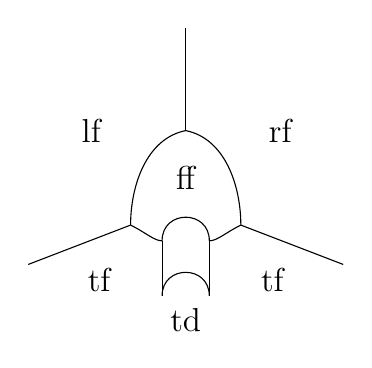
\begin{tikzpicture}
\draw (0,0.7) -- (0,2);
\draw (-0.7,-0.5) -- (-2,-1);
\draw (0.7,-0.5) -- (2,-1);
\draw (0,0.7) .. controls (-0.5,0.6) and (-0.7,0) .. (-0.7,-0.5);
\draw (0,0.7) .. controls (0.5,0.6) and (0.7,0) .. (0.7,-0.5);
\draw (-0.7,-0.5) .. controls (-0.5,-0.6) and (-0.4,-0.7) .. (-0.3,-0.7);
\draw (0.7,-0.5) .. controls (0.5,-0.6) and (0.4,-0.7) .. (0.3,-0.7);
\draw (-0.3,-0.7) .. controls (-0.3,-0.3) and (0.3,-0.3) .. (0.3,-0.7);
\draw (-0.3,-1.4) .. controls (-0.3,-1) and (0.3,-1) .. (0.3,-1.4);
\draw (0.3,-0.7) -- (0.3,-1.4);
\draw (-0.3,-0.7) -- (-0.3,-1.4);
\node at (1.2,0.7) {\large{rf}};
\node at (-1.2,0.7) {\large{lf}};
\node at (1.1, -1.2) {\large{tf}};
\node at (-1.1, -1.2) {\large{tf}};
\node at (0, -1.7) {\large{td}};
\node at (0,0.1) {\large{ff}};
\end{tikzpicture}
\end{center}
\label{blowup}
\caption{The blowup space $\mathscr{M}^2_b$.}
\end{figure}

Projective coordinates on $\mathcal{M}_b$ are given as follows. 
Near the top corner of ff away from tf the projective coordinates are given by
\begin{align}\label{top-coord}
\rho=\frac{1}{\mu}, \  \xi=\frac{x}{\rho}, \ \widetilde{\xi}=\frac{y}{\rho},
\end{align}

where in these coordinates $\rho, \xi, \widetilde{\xi}$ are the defining functions of 
the faces ff, lf and rf respectively. For the bottom corner of ff away from rf the 
projective coordinates are given by
\begin{align}\label{right-coord}
\tau=(\mu y)^{-1}, \ s=\frac{x}{y}, \ y,
\end{align}

where in these coordinates $\tau, s, y$ are the defining functions of tf, lf and ff respectively. 
For the bottom corner of ff away from lf the projective coordinates are obtained by interchanging 
the roles of $x$ and $y$. The projective coordinates on $\mathcal{M}_b$ near the top of td away 
from tf are given by 
\begin{align}\label{d-coord}
\eta=\tau, \ S =\frac{s-1}{\eta}, y.
\end{align}

In these coordinates tf is the face in the limit $|S|\to \infty$, ff and td are defined by 
$y, \eta$, respectively. The blowup blowup-space $\mathcal{M}_b$ is related to the original 
space $\R_+\times \R_+^2$ via the obvious `blow-down map'
\[
\beta: \mathcal{M}_b\to \R_+\times \R_+^2,
\]
which is in local coordinates simply the coordinate change back to $(1/\mu, x,y)$. 
The blowup $\mathscr{M}^2_b$ is similar to the blowup space construction for incomplete
conical singularities by Mooers \cite{Moo:HKA} with the difference that here the 
blowup is not parabolic in $\mu^{-1}-$direction.

One can easily check in local projective coordinates above that the 
kernels $K_+$ and $K_\R$ both lift to polyhomogeneous 
distributions on $\mathscr{M}^2_b$, the latter being conormal to $\beta^*\{x=y\}$. 
Put for any $k\in \N_0$ 
\begin{align}
E_k:=\{(j,0)\in \N\times \N \mid j \geq k\}.
\end{align}

Then the index set of $\beta^*K_\R$ is given by $E_1$ at ff and td, 
by $E_0$ at rf and lf. The index sets of $K_+$ are the same at ff, rf and lf, 
and given by $E_{\infty}$ at tf, which simply means that 
$\beta^*K_+$ is vanishing to infinite order at the temporal face tf. 

We denote by $\mathscr{A}_{\textup{phg}}^{l,p,E_{\textup{lf}}, 
E_{\textup{rf}}}(\mathscr{M}^2_b, \beta^*\{x=y\})$ 
the space of polyhomogeneous distributions on
$\mathscr{M}^2_b$ conormal up to $\beta^*\{x=y\}$, with index set
$E_l, l\in \N$ at ff, index sets $(E_{\textup{lf}}, E_{\textup{rf}})$ 
at lf and rf, respectively, and the index set $E_p$ at tf. The 
space $\mathscr{A}_{\textup{phg}}^{l,p,E_{\textup{lf}}, 
E_{\textup{rf}}}(\mathscr{M}^2_b)$ denotes the subspace 
of polyhomogeneous distributions that are smooth across $\beta^*\{x=y\}$. Clearly, 
$K_\R \in \mathscr{A}_{\textup{phg}}^{1,1,E_0, E_0}(\mathscr{M}^2_b,\beta^*\{x=y\})$, 
as the Schwartz kernel of an elliptic operator $(\Delta^\R +\mu^2)^{-1}$ inside the 
strongly parametric calculus. Moreover $K_+ \in \mathscr{A}_{\textup{phg}}^{1,\infty ,E_0, E_0}
(\mathscr{M}^2_b)$.

We need to establish polyhomogeneity for the various compositions 
of $K_+$ and $K_\R$, or more generally for any 
$K_A \in \mathscr{A}_{\textup{phg}}^{l,p,E_{\textup{lf}}, E_{\textup{rf}}}(\mathscr{M}^2_b)$ 
and $K_B \in \mathscr{A}_{\textup{phg}}^{l',\infty,E'_{\textup{lf}}, E'_{\textup{rf}}}(\mathscr{M}^2_b)$.  
We employ the pushforward theorem in the following way. Consider the composition
\begin{equation}
K_{C}(x,y;\mu) = \int_{\R_+} K_A(x,z;\mu) K_B(z,y;\mu) dz.
\label{comp1}
\end{equation}
This expression can be rephrased as follows. 
 Consider the triple-space $R^+_{1/\mu}\times (\R_+)^3_{(x,z,y)}$, and the three projections
\begin{equation}
\begin{split}
&\pi_C :R^+_{1/\mu}\times (\R_+)^3_{(x,z,y)} \to R^+_{1/\mu}\times (\R_+)^2_{(x,y)}, \\
&\pi_\Delta: R^+_{1/\mu}\times (\R_+)^3_{(x,z,y)} \to R^+_{1/\mu}\times (\R_+)^2_{(x,z)}, \\
&\pi_R: R^+_{1/\mu}\times (\R_+)^3_{(x,z,y)} \to R^+_{1/\mu}\times (\R_+)^2_{(z,y)}.
\end{split}
\label{projections}
\end{equation} 
Assuming that all kernels are extended to vanish for $\mu^{-1}<0$, 
and reinterpreting them as densities in a suitable way specified below, we can rewrite \eqref{comp1} as
\[
K_C = (\pi_C)_* \left( \pi_\Delta^* K_A  \pi_R^* K_B \right).
\]

The basic idea is a construction of a triple-space $\mathscr{M}^3_b$,
which is a blowup of $R^+_{1/\mu}\times (\R_+)^3_{(x,z,y)}$ obtained 
by a sequence of blowups, such that there are maps
\[
\Pi_\Delta, \Pi_C, \Pi_R:  \mathscr{M}^3_b \longrightarrow 
[\R^+_{1/\mu}\times \R_+^2, \mathscr{A}]=:  \mathscr{M}^2_{rb}
\]
which `cover' the three projections defined above. Note that the 
space $\mathscr{M}^2_{rb}$ is not the full blowup $ \mathscr{M}^2_{b}$, 
since the diagonal $\mathscr{D}$ is not blown up in $\mathscr{M}^2_{rb}$, 
which we therefore refer to as the reduced blowup space.

Lifting the composition to these spaces leads to the key formula
\begin{equation}
\kappa_C = (\Pi_C)_* \left( \Pi_\Delta^* \kappa_A  \Pi_R^* \kappa_B \right).
\label{comp2}
\end{equation}
Thus it suffices to show that if $\kappa_A$ and $\kappa_B$ are polyhomogeneous, then their lifts to $M^3_h$
are also polyhomogeneous, and so too the product of these lifts, and most importantly, that the pushforward
by $\Pi_C$ of this product is again polyhomogeneous on $M^2_h$.  

% REPHRASE AS IT COMES FROM THE JOINT WORK WITH RAFE

In order to state the pushforward theorem, introduce some terminology.  
Let $X$ and $X'$ be two compact manifolds with corners, and let $f: X \to X'$ 
be a smooth map.  Let $\{H_i\}$ and $\{H_j'\}$ be enumerations of the codimension one boundary faces of $X$ and $X'$,
respectively, and let $\rho_i$, $\rho_j'$ be global defining functions for $H_i$, resp.\ $H_j'$. We say that the map $f$
is a $b$-map if $f^* \rho_j'$ is a smooth nonvanishing multiple of some product of nonnegative integer powers
of the defining functions $\rho_i$, or symbolically,
\[
f^* \rho_i' = A_{ij} \prod_i \rho_j^{e(i,j)}, \quad A_{ij} > 0,\ e(i,j) \in \mathbb{N} \cup \{0\}.
\]
This simply means that $f$ respects the boundary structure of these two spaces, and in particular maps each $H_i$ into some $H_j'$ 
with constant normal order of vanishing along the entire face. 

The map $f$ is called a $b$-submersion if $f_*$ induces a surjective map between the $b$-tangent bundles
of $X$ and $X'$. (The $b$-tangent space at a point $p$ of $\partial X$ on a codimension  $k$ corner is spanned locally by  the
sections $x_1 \partial_{x_1}, \ldots, x_k \partial_{x_k}, \partial_{y_j}$, where $x_1, \ldots, x_k$ are the defining functions for the faces
meeting at $p$ and the $y_j$ are local coordinates on the corner through $p$.)  If, in addition, the matrix $e(i,j)$ defined
above has the property that for each $j$ there is at most one $i$ such that $e(i,j) \neq 0$ (this condition simply means
that each hypersurface face $H_i$ in $X$ gets mapped into \emph{at most one} $H_j'$ in $X'$, or in other words, no
hypersurface in $X$ gets mapped to a corner in $X'$), then $f$ is called a $b$-fibration. 

Suppose that $\nu_0$ is a density on $X$ which is smooth up to all boundary faces and everywhere nonvanishing. 
A smooth $b$-density $\nu_b$ is, by definition, any density of the form $\nu_b =\nu_0 (\Pi \rho_i)^{-1}$.  
Let us fix smooth nonvanishing $b$-densities $\nu_b$ on $X$ and $\nu_b'$ on $X'$. 
\begin{prop}[The Pushforward Theorem]
Let $u$ be a polyhomogeneous function on $X$ with index sets  $E_j$ the faces $H_j$ of $X$.  Suppose that each $(z,p) \in E_j$
has $\mbox{Re}\, z > 0$ if the index $j$ satisfies $e(i,j) = 0$ for all $j$ (which means that $H_j$ is mapped to the interior of $X'$).
Then the pushforward $f_* (u \nu_b)$ is well-defined and equals $h \nu_b'$ where $h$ is polyhomogeneous on $X'$ and has
an index family $f_b(\mathcal{E})$ given by an explicit formula in terms of the index family $\mathcal{E}$ for $X$.
\end{prop}
Rather than giving the formula for the image index set in generality, let us describe it slightly informally but specifically
enough for the present situation.  If $H_{j_1}$ and $H_{j_2}$ are both mapped to a face $H_i'$, and if $H_{j_1} \cap H_{j_2} = \emptyset$,
then they contribute the index set $E_{j_1} + E_{j_2}$ to $H_i'$. If they do intersect, however, then the contribution is the
extended union $E_{j_1} \overline{\cup} E_{j_2}$
\begin{align*}
E_{j_1} \overline{\cup} E_{j_2} := E_{j_1} \cup E_{j_2} \cup \{((z, p + q + 1): \exists \, (z,p) \in E_{j_1},\ 
\mbox{and}\  (z,q) \in E_{j_2} \}.
\end{align*}

We then 
have the following fundamental composition result.

\begin{prop}
\label{composition}
For index sets $E_{\lf}$ and $E'_{\rf}$ such that $E_{\lf}+E'_{\rf}>-1$, we have
\[
\mathscr{A}_{\textup{phg}}^{l,p,E_{\textup{lf}}, E_{\textup{rf}}}(\mathscr{M}^2_b) \circ 
\mathscr{A}_{\textup{phg}}^{l',\infty,E'_{\textup{lf}}, E'_{\textup{rf}}}(\mathscr{M}^2_b,\beta^*\{x=y\}) \subset 
\mathscr{A}_{\textup{phg}}^{l+l'+1,\infty, E'_{\textup{lf}}, E_{\textup{rf}}}(\mathscr{M}^2_b).
\]
\end{prop}

\begin{proof}
Consider $K_A \in \mathscr{A}_{\textup{phg}}^{l,p,E_{\textup{lf}}, E_{\textup{rf}}}(\mathscr{M}^2_b)$ 
and $K_B \in \mathscr{A}_{\textup{phg}}^{l',\infty,E'_{\textup{lf}}, E'_{\textup{rf}}}(\mathscr{M}^2_b,\beta^*\{x=y\})$. 
We are interested in the polyhomogeneous expansion of their composition
\[
K_C (x,y;\mu) = \int_{\R_+} K_A(x,z;\mu) K_B(z,y;\mu) dz.
\]

The aformentioned triple space $\mathscr{M}^3_b$ is constructed by a sequence of blowups,
where the steps are dictated strictly by the requirements that the maps
$\pi_\Delta, \pi_C, \pi_R$ all lift to $b$-fibrations $\Pi_\Delta, \Pi_C, \Pi_R$. The construction 
is reminiscent of the triple space construction for the heat space calculus for conical 
singularities, see \cite{Moo:HKA}, but differs from the latter since there is no convolution 
in the parameter $\mu^{-1}$ variable and the blowups are not parabolic in the $\mu^{-1}$
direction. First we blow up the submanifold
\[
F=\{\mu = \infty, x=z=y=0\}.
\]
Then we blow up the resulting space $[R^+_{1/\mu}\times (\R_+)^3_{(x,z,y)}, F]$ at the 
lifts of each of the three submanifolds
\begin{equation}
\begin{split}
F_C&=\{\mu = \infty, x=y=0\}, \\
F_\Delta&=\{\mu = \infty, z=y=0\}, \\
F_R&=\{\mu = \infty, x=z=0\}.
\end{split}
\end{equation} 
Thus altogether,
\[
\mathscr{M}^3_b := \left[R^+_{1/\mu}\times (\R_+)^3_{(x,z,y)}, F; F_C, F_\Delta, F_R\right].
\]

If we ignore the $\mu^{-1}-$direction, the spatial part of $\mathscr{M}^3_b$ is 
exactly the same as the triple space appearing in the elliptic theory of edge operators, 
see \cite{Maz:ETO}, which can be visualized as in Figure 5.
\begin{figure}[h]
\begin{center}
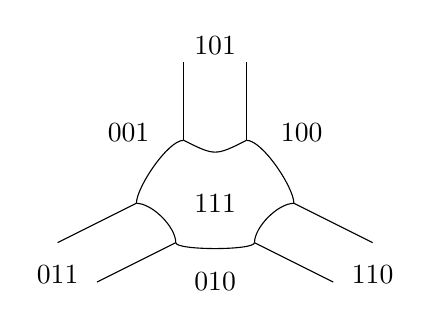
\begin{tikzpicture}

\draw  (-1,0) .. controls (-0.8,0) and (-0.5,-0.3) .. (-0.5,-0.5);
\draw  (1,0) .. controls (0.8,0) and (0.5,-0.3) .. (0.5,-0.5);
\draw  (-0.4,0.8) .. controls (0,0.6) and (0,0.6) .. (0.4,0.8);

\draw  (-1,0) -- (-2,-0.5);
\draw  (-0.5,-0.5) -- (-1.5,-1);

\draw  (1,0) -- (2,-0.5);
\draw  (0.5,-0.5) -- (1.5,-1);

\draw   (-0.4,0.8)  --  (-0.4,1.8) ;
\draw   (0.4,0.8)  --  (0.4,1.8);

\draw  (-1,0) .. controls (-1,0.2) and (-0.6,0.8) ..  (-0.4,0.8);
\draw  (1,0) .. controls (1,0.2) and (0.6,0.8) ..  (0.4,0.8);
\draw  (-0.5,-0.5) .. controls (-0.5,-0.6) and (0.5,-0.6) .. (0.5,-0.5);

\node at (0,0) {111};
\node at (-2,-0.9) {011};
\node at (2,-0.9) {110};
\node at (0,2) {101};
\node at (0,-1) {010};
\node at (-1.1,0.9) {001};
\node at (1.1,0.9) {100};
\end{tikzpicture}
\end{center}
\label{triple-space}
\caption{The spatial component of the triple space $\mathscr{M}^3_b$.}
\end{figure} 

% REPHRASE AS IT COMES FROM THE JOINT WORK WITH RAFE

Here, $(101), (011)$ and $(110)$ label the boundary faces created by blowing up $F_C, F_\Delta$ and $F_R$, respectively. 
The face $(111)$ is the front face introduced by blowing up $F$. We denote the defining function for the face $(ijk)$  
by $\rho_{ijk}$. The triple space comes with a natural blowdown map 
$\beta^{(3)}: \mathscr{M}^3_b \to \R_+ \times (\R_+)^3$. 

Now recall the projections $\pi_C$, $\pi_\Delta$ and $\pi_R$ defined in \eqref{projections}.  
These induce projections $\Pi_C$, $\Pi_\Delta$ and $\Pi_R$ from 
$\mathscr{M}^3_b$ to the reduced blowup space $\mathscr{M}^2_{rb}$. 
It is not hard to check that the choice of submanifolds $F, F_{\Delta,R,C}$ that have been blown up ensures that these 
projections are in fact $b$-fibrations. 

Denote the defining functions for the right, front and left faces of each copy of $\mathscr{M}^2_{rb}$ by 
$\{\rho_{10}, \rho_{11}, \rho_{01}\}$, respectively.  These lift via the projections according to the following rules
\begin{equation}
\begin{split}
&\Pi_C^*(\rho_{ij})=\rho_{i0j}\rho_{i1j}, \\ 
&\Pi_\Delta^*(\rho_{ij})=\rho_{ij0}\rho_{ij1}, \\ 
&\Pi_R^*(\rho_{ij})=\rho_{0ij}\rho_{1ij}.
\end{split}
\label{RLC}
\end{equation}

Now consider the behaviour in the parameter $\mu^{-1}$direction. Let $\tau$ be the defining function 
for the boundary face in $\mathscr{M}^3_b$ corresponding to $\{\mu=\infty\}$. 
Then we find 
\begin{align}
\label{beta-tau}
(\beta^{(3)})^*(\mu^{-1}) = \tau \rho_{111} \rho_{110} \rho_{101} \rho_{011}.
\end{align} 

Let $\beta^{(2)}: \mathscr{M}^2_{rb} \to \R_+ \times \R_+^2$ be the 
blowdown map for the reduced blowup space. The lifts $\left(\beta^{(2)}\right)^*(\mu^{-1})$ 
to $\Pi_\Delta(M^3_{rh})$, $\Pi_R(\mathscr{M}^3_b)$ and $\Pi_C(\mathscr{M}^3_b)$ are 
equal to $T \rho_{11}^2$, where $T$ is the defining function 
for the temporal face tf in $\mathscr{M}^2_{rb}$. Note 
\[
\Pi^*_{C,\Delta,R} \circ \left(\beta^{(2)}\right)^* = \left(\beta^{(3)}\right)^* \circ \pi^*_{C,\Delta,R}.
\]
Consequently, in view of \eqref{RLC} and \eqref{beta-tau}, we conclude
\begin{equation}
\begin{split}
&\Pi_C^*(T)=\tau \rho_{110} \rho_{011}, \\
&\Pi_\Delta^*(T)=\tau \rho_{101} \rho_{011}, \\
&\Pi_R^*(T)=\tau \rho_{101} \rho_{110}.
\end{split}
\end{equation}

Using these data, we now derive the anticipated composition formula. 
Consider again $K_A \in \mathscr{A}_{\textup{phg}}^{l,p,E_{\textup{rf}}, E_{\textup{rf}}}(\mathscr{M}^2_b)$ 
and $K_B \in \mathscr{A}_{\textup{phg}}^{l',\infty,E'_{\textup{rf}}, E'_{\textup{rf}}}(\mathscr{M}^2_b,\beta^*\{x=y\})$. 
We write $t:=\mu^{-1}$ and reinterpret both kernels as `right densities', 
$K_A(x,z;t) dz$ and $K_B(z,y;t) dy$. Then their product on $\R^+_t \times (\R_+)^3_{(x,z,y)}$ is
\[
K_A(x,z;t) K_B(z,y;t) dz \, dy.
\]
The integral over $dz$ gives $K_{A\circ B}(x,y;t) dy$. To put this into the same form required
in the pushforward theorem, multiply this expression by $dt \, dx$. 

Blowing up a submanifold of codimension $n$ amounts in local coordinates to introducing polar coordinates, so that 
the coordinate transformation of a density leads to $(n-1)^{\mathrm{st}}$ power of the radial function, which 
is the defining function of the corresponding front face. Hence we compute the lift
\begin{equation}
\begin{split}
&(\beta^{(3)})^* (dt \, dx \, dz \, dy) \\
&=\rho_{111}^{3}\rho_{101}^{2}\rho_{110}^{2}\rho_{011}^{2} 
\nu^{(3)}=\rho_{111}^{3}\rho_{101}^{2}\rho_{110}^{2}\rho_{011}^{2} 
\tau \left( \Pi \rho_{ijk} \right) \nu^{(3)}_b,
\end{split}
\label{lift1}
\end{equation}

where $\nu^{(3)}$ is a density on $\mathscr{M}^3_b$, smooth up to all boundary faces and everywhere 
nonvanishing; $\nu^{(3)}_b$ is a $b$-density, obtained from $\nu^{(3)}$ by dividing 
by a product of all defining functions on $\mathscr{M}^3_b$; 
and $\left( \Pi \rho_{ijk} \right)$ is a product over all $(ijk)\in \{0,1\}^3$. 
Furthermore, the infinite order vanishing of $\kappa_A= (\beta^{(2)})^* K_A$ and 
$\kappa_B =  (\beta^{(2)})^* K_B$ at $T=0$ 
implies that the product of the lifts
vanishes to infinite order in $\tau \rho_{110} \rho_{101} \rho_{011}$. Altogether, we obtain that
\[
\left(\Pi_\Delta^*\kappa_A\right) \left(\Pi_R^*\kappa_B\right) (\beta^{(3)})^* (dt \, dx \, dz \, dy)  
 =\rho_{111}^{\ell + \ell' + 3} \left( \Pi \rho_{ijk} \right) G \nu_b^{(3)},
\]

where $G$ is a bounded polyhomogeneous function on $\mathscr{M}^3_b$, 
vanishing to infinite order in $(\tau \rho_{110} \rho_{101} \rho_{011})$, 
with index sets $E'_{\lf}$, $E_{\rf}$ and $E_{\lf} + E'_{\rf}$ 
at the faces $(001)$, $(100)$ and $(010)$, respectively. 

Note that since $\kappa_A$ does not vanish to infinite order on td in $\mathscr{M}^2_b$, 
the lift $\Pi_\Delta^* \kappa_A$ is not polyhomogeneous
on $\mathscr{M}^3_b$. Fortunately, the other factor $\kappa_B$ 
does vanish to infinite order there, and hence the product 
$\Pi_\Delta^*\kappa_A \cdot \Pi_R^*\kappa_B$ is indeed polyhomogeneous 
on $\mathscr{M}^3_b$. Applying the Pushforward Theorem now gives
\begin{equation}
\begin{split}
&\left(\Pi_C\right)_*\left(\left(\Pi_\Delta^*\kappa_A\right) \left(\Pi_R^*\kappa_B\right) 
(\beta^{(3)})^* (dt \, dx \, dz \, dy)\right) \\
& = \left(\beta^{(2)}\right)^*\left(K_{A\circ B}x,y;t)dt \, dx \, dy\right) \\
&= (\rho_{11} \rho_{10} \rho_{01} T) \, G' \, \nu^{(2)}_b,
\end{split}
\label{lift3}
\end{equation}
where $\nu^{(2)}_b$ is a $b$-density on $\mathscr{M}^2_{rb}$ 
and $G'$ is a bouned polyhomogeneous function on $\mathscr{M}^2_{rb}$, 
which vanishes to infinite order in $T$, is of leading order $(\ell + \ell'+3)$ at 
the front face and has the index sets $(E'_{\lf}, E_{\rf})$ 
at the left and right boundary faces. By \cite[Proposition B7.20]{EMM:ROT} the 
pushforward is again smooth across $\beta^*\{x=y\}$.

Note first that the pushforward by $\Pi_C$ does not introduce logarithmic 
terms in the front face expansion of $\kappa_{A\circ B}$, since 
the kernel on $\mathscr{M}^2_{rb}$ is vanishing to infinite order at $(101)$. 
Hence, for $\kappa_A$ and $\kappa_B$ with integer exponents in their front face expansions, 
same holds for their composition.

By an argument similar to \eqref{lift1}, we compute
\begin{equation}
\begin{split}
\left(\beta^{(2)}\right)^*(dt \, dx\, dy)=\rho_{11}^{2} \left(\rho_{10}\rho_{11}\rho_{01} T\right) \nu^{(2)}_b .
\end{split}
\label{lift4}
\end{equation}
Consequently, combining \eqref{lift3} and \eqref{lift4}, we deduce that 
$(\beta^{(2)})^* K_{A \circ B}=\kappa_{A\circ B}$ 
vanishes to infinite order in $T$, is of leading order $(\ell + \ell'+1)$ at 
the front face and has the index sets $(E'_{\lf}, E_{\rf})$ 
at the left and right boundary faces. 
This proves the statement.
\end{proof}

\begin{prop}
\label{trace-boundary}
For any $K \in 
\mathscr{A}_{\textup{phg}}^{l,\infty,E_{\textup{lf}}, E_{\textup{rf}}}(\mathscr{M}^2_b)$, 
and any cutoff function $\phi \in C^\infty_c(\R_+)$ with $\phi \equiv 1$ 
in an open neighborhood of zero, we find for $(E_{\textup{lf}} + E_{\textup{rf}} + 1) >-1$ 
\begin{align}
\textup{Tr} (K\phi) = \int_{\R_+} K(x,x; \mu)\phi(x) dx \sim \sum_{j=0}^\infty 
a_j \mu^{-(l+1)-j}, \ \mu \to \infty.
\end{align} 
\end{prop}

\begin{proof}
The lift $\beta^* K$ restricts to a polyhomogeneous distribution on
$\mathscr{B}:=\beta^*\{x=y\} \subset \mathscr{M}^2_b$, which itself is a blowup of 
$\R^+_{1/\mu} \times \R^+_x$ at $(0,0)$ with the blowdown map denoted 
by $\beta_{\mathscr{B}}$. We refer to the restrictions of ff, lf and td in 
$\mathscr{M}^2_b$ to $\mathscr{B}$ as the front face, left face and 
temporal diagonal again. 

The restriction of $\beta^*K$ to $\mathscr{B}$ is polyhomogeneous 
with the index set $E_l$ at the front face, index set $(E_{\lf}+ E_{\rf})$ 
at the left face and vanishes to infinite order at the temporal diagonal.
Consider the projection $\pi: \R^+_{1/\mu} \times \R^+_x$. Then ($t=1/\mu$)
\begin{align*}
(\pi \circ \beta_{\mathscr{B}})_* \left( \beta^*(K\phi)|_{\mathscr{B}} 
\beta^*_{\mathscr{B}}(dt \, dx)\right) 
 \int_{\R_+} K(x,x;\mu) \phi(x) dx \, dt.
\end{align*}
Note that 
\[
\beta^*(K\phi)|_{\mathscr{B}} \beta^*_{\mathscr{B}}(dt \, dx)  
= \rho_\ff^{l+2} G \nu_b.
\]
where $\nu_b$ is a $b$-density on $\mathscr{B}$, $\rho_\ff$ is the 
defining function of the front face and $G$ is a bounded polyhomogeneous 
distribution with index set $(E_{\textup{lf}} + E_{\textup{rf}} + 1)$ 
at the left face and vanishes to infinite order at the temporal diagonal 
in $\mathscr{B}$. By the pushforward theorem we find
\begin{align*}
(\pi \circ \beta_{\mathscr{B}})_* \left( \beta^*(K\phi)|_{\mathscr{B}} 
\beta^*_{\mathscr{B}}(dt \, dx)\right) = 
(\pi \circ \beta_{\mathscr{B}})_* \left( \rho_\ff^{l+2} G \nu_b \right) 
\sim \sum_{j=0}^\infty t^{(l+2)+j} \frac{dt}{t}.
\end{align*}
This proves the statement.
\end{proof}

We can now employ Proposition \ref{composition} together with Proposition \ref{trace-boundary}
in order to derive a polyhomogeneous expansion of the finite sum
\[
\sum_{j=0}^{M-1} (-1)^j \psi \left( \left[K_\theta \lambda(V,W)\right]^j 
K_\theta -  \left[K_\R \lambda(V,W)\right]^j K_\R \right) \phi, 
\]
Recall the notation $\lambda(V,W)=\lambda^2\widetilde{V}_\psi + W_\psi$
and $\mu^2=\lambda^2V(0)+z^2$. Hence, multiplying out the sum above leads to a finite number of 
summands of the form $K(j,p,q)$, which are given by a convolution of 
$(j+1), j\leq (M-1)$ kernels $K_\R, K_+$, with at least one $K_+$, 
$p\leq j$ times $\lambda^2 \widetilde{V}_\psi$ and $q\leq j$ times 
$W_\psi$. Note that $\widetilde{V}_\psi(x)=O(x)$ as $x\to 0$, and is smooth so that 
\begin{align*}
K_\R\widetilde{V}_\psi\in  \mathscr{A}_{\textup{phg}}^{2,1,E_1, E_0}(\mathscr{M}^2_b, \beta^*\{x=y\}),
\quad K_+\widetilde{V}_\psi\in  \mathscr{A}_{\textup{phg}}^{2,\infty,E_1, E_0}(\mathscr{M}^2_b). 
\end{align*}
Consequently we find by Proposition \ref{composition}
\[
K(j,p,q) \in \lambda^{2p} \mathscr{A}_{\textup{phg}}^{2j+1+p,\infty,E_0, 
E_0}(\mathscr{M}^2_b).
\]
Proposition \ref{trace-boundary} now implies 
\[
\textup{Tr} K(j,p,q) \sim \sum_{i=0}^\infty a_i \frac{\lambda^{2p}}
{\mu^{2(j+1)+p+i}} =: \sum_{i=0}^\infty a_i^{jp} (\lambda, z),
\]
where each $a_i^{jp}$ is homogeneous in $(\lambda, z)$ of homogeneity 
degree $(p-2(j+1)-i)$. Consequently, overall we obtain
\begin{equation}
\label{boundary-expansion}
 \begin{split}
\Tr \sum_{j=0}^{M-1} (-1)^j \psi \left( \left[K_\theta \lambda(V,W)\right]^j 
K_\theta -  \left[K_\R \lambda(V,W)\right]^j K_\R \right) \phi \\ 
\sim \sum_{i=0}^\infty e_i(\lambda,z), \ |(\lambda,z)| \to \infty,
 \end{split}
\end{equation}
where each $e_i\in C^{\infty}(\R^2_+\backslash \{(0,0)\})$ is homogeneous
of order $(-2-i)$ jointly in both variables.

Comparing to \eqref{interior-expansion}, we see that the leading term in the 
polyhomogeneous expansion of $\Tr(\Delta_\lambda+z^2)^{-1}$ indeed 
comes from the interior. Summarizing \eqref{boundary-expansion} with the polyhomogeneous expansion of 
the interior parametrix in \eqref{interior-expansion} and \eqref{remainder-expansion} we finally arrive at 
our first main result, Proposition \ref{phg-trace}.

\begin{prop}
\label{phg-trace2}
The resolvent $(\Delta_\lambda+z^2)^{-1}$ is trace class for $z\geq z_0$, 
and its trace admits the following polyhomogeneous expansion 
\begin{align*}
\partial_\lambda^{\A}\partial_z^{\beta}
\Tr(\Delta_\lambda+z^2)^{-1} \sim \sum_{i=0}^\infty h_i (\lambda,z), \ |(\lambda,z)| \to \infty,
\end{align*}
where $\gamma_i:=(i+\A+\beta +1)$ and each $h_i\in C^{\infty}(\R^2_+\backslash \{(0,0)\})$
is homogeneous of order $(-\gamma_i)$ jointly in both variables. 
\end{prop}

As an application of the polyhomogeneity of the resolvent trace 
we now clarify in which sense the trace expansions 
of $\Tr(\Delta_\lambda+z^2)^{-2}$ sum up to the trace expansion 
of $\Tr(\Delta+z^2)^{-2}$. Note that $\Tr(\Delta_\lambda+z^2)^{-2}=O(z^{-3})$, 
whereas $\Tr(\Delta+z^2)^{-2}=O(z^{-2})$, as $z\to \infty$. 
So the trace expansions clearly do not sum up in an obvious way.
We employ the Euler Maclaurin formula \eqref{EM} 
and find for $z\geq z_0$ sufficiently large
\begin{equation}
\begin{split}
\sum_{\lambda=1}^{N} \Tr(\Delta_\lambda+z^2)^{-2} &=
\int_1^N \Tr(\Delta_\lambda+z^2)^{-2} d\lambda \\
&+ \sum_{k=1}^M \frac{B_{2k}}{(2k)!} \,
\partial_\lambda^{(2k-1)}\Tr(\Delta_\lambda+z^2)^{-2}|_{\lambda=N} \\
&- \sum_{k=1}^M \frac{B_{2k}}{(2k)!}  \,
\partial_\lambda^{(2k-1)}\Tr(\Delta_\lambda+z^2)^{-2}|_{\lambda=1} \\ 
&+ \frac{1}{(2M+1)!} \int_1^N B_{2M+1}(\lambda-[\lambda]) \,
\partial_\lambda^{(2M+1)}\Tr(\Delta_\lambda+z^2)^{-2} d\lambda \\ &+ 
\frac{1}{2}(\Tr(\Delta_1+z^2)^{-2}+\Tr(\Delta_N+z^2)^{-2}),
\end{split}
\end{equation}
where $B_j$ denotes the $j$-th Bernoulli number, $B_j(x)$ the $j$-th Bernoulli 
polynomial. Using Proposition \ref{phg-trace2} we consider the limit $N\to \infty$ and find
\begin{equation}
\label{EM2}
\begin{split}
\sum_{\lambda=1}^{\infty} \Tr(\Delta_\lambda+z^2)^{-2} &=
\int_1^\infty \Tr(\Delta_\lambda+z^2)^{-2} d\lambda \\
&+ \frac{1}{2}\Tr(\Delta_1+z^2)^{-2} - \sum_{k=1}^M \frac{B_{2k}}{(2k)!} \, 
\partial_\lambda^{(2k-1)}\Tr(\Delta_\lambda+z^2)^{-2}|_{\lambda=1} \\ 
&+ \frac{1}{(2M+1)!} \int_1^\infty B_{2M+1}(\lambda-[\lambda]) \,
\partial_\lambda^{(2M+1)}\Tr(\Delta_\lambda+z^2)^{-2} d\lambda.
\end{split}
\end{equation}
We need to establish asymptotic behaviour of each of the terms above as $z\to \infty$.
The standard resolvent trace expansion yields 
\begin{equation}
\label{exp1}
\begin{split}
\frac{1}{2}\Tr(\Delta_1+z^2)^{-2}  - \sum_{k=1}^M \frac{B_{2k}}{(2k)!} \, 
\partial_\lambda^{(2k-1)}\Tr(\Delta_\lambda+z^2)^{-2}|_{\lambda=1} 
\sim \sum_{i=0}^{\infty} a_i z^{-3-i}, \ z\to \infty.
\end{split}
\end{equation}
Moreover, Proposition \ref{phg-trace2} implies
\begin{equation}
\label{exp2}
\begin{split}
\frac{1}{(2M+1)!} \int_1^\infty B_{2M+1}(\lambda-[\lambda]) \, 
\partial_\lambda^{(2M+1)}\Tr(\Delta_\lambda+z^2)^{-2} d\lambda\\
\leq C \cdot \int_1^\infty (\lambda+z)^{-4-2M} d\lambda =O(z^{-3-2M}), \ z\to\infty.
\end{split}
\end{equation}
It remains to derive an asymptotic expansion for the second term in \eqref{EM2}.
Proposition \ref{phg-trace2} implies
\begin{align*}
\Tr(\Delta_\lambda+z^2)^{-2} = (2z)^{-1} \partial_z
\Tr(\Delta_\lambda+z^2)^{-1} \sim \sum_{i=0}^\infty h_i (\lambda,z), \ |(\lambda,z)| \to \infty,
\end{align*}
where $\gamma_i:=(i+3)$ and each $h_i\in C^{\infty}(\R^2_+\backslash \{(0,0)\})$
is homogeneous of order $(-\gamma_i)$ jointly in both variables. 
The asymptotic expansion of the second term in \eqref{EM2}
follows from the following simple calculation
\begin{align*}
\int_1^\infty h_i(\lambda, z) \, d\lambda = 
z^{-\gamma_i} \int_1^\infty h_i(\lambda / z, 1) \, d\lambda =
z^{-\gamma_i + 1} \int_1^\infty h_i(\nu, 1) \, d\nu,
\end{align*}
where the $\nu$-integral is finite, since as a consequence of 
smoothness of $h_i(1,\cdot)$ at $z=0$ and homogeneity, $h(\nu,1) = O(\nu^{-\gamma_i}), \gamma_i\geq 3$, 
see Remark \ref{reg-int-remark} below.
This proves our second main result
\begin{theorem}
\begin{align}
\Tr(\Delta+z^2)^{-2} \equiv \sum_{\lambda=-\infty}^{\infty}\Tr(\Delta_\lambda+z^2)^{-2} 
\sim \sum_{k=2}^\infty a_k z^{-k}, \ z \to \infty. 
\end{align}
\end{theorem}


%**************************************************************************
\section{Fubini theorem for regularized integrals}
%**************************************************************************
The following Fubini-type result for homogeneous functions is 
the main technical tool for proving the general Fubini Theorem \ref{fubini}
for polyhomogeneous functions.

\begin{theorem}
Let $f_{\A}\in C^{\infty}(\R_+^2 \backslash \{(0,0)\})$ be homogeneous of degree $\A \in \C$ in both variables jointly. Then the following Fubini-identity holds
\begin{equation}
\label{27-1}
\regint\limits_1^\infty \regint\limits_1^\infty f_{\A}(x,y) dy \, dx - 
\regint\limits_1^\infty \regint\limits_1^\infty f_{\A}(x,y) dx \, dy = 
\left\{
\begin{split}
\regint\limits_0^\infty &f_{\A}(1,y) \log(y) dy, \ &\A=-2, \\
&0, &\A\neq -2.
\end{split}
\right.
\end{equation}
\end{theorem}

\begin{remark}\label{reg-int-remark}
The smoothness of $f_\A$ on $\R^2_+\backslash\{(0,0)\}$
implies the smoothness of $f_\A(1,\cdot)$ and $f_\A(\cdot, 1)$
up to $0$. Furthermore, the homogeneity and the Taylor expansion 
of $f_\A(\cdot, 1)$ at $0$ give for $y \to \infty$
\begin{equation}
\label{27-2}
f_\A(1,y)=y^\A f_\A(1/y,1)
\sim \sum_{j=0}^\infty \frac{\partial_1^{(j)}f_\A(0,1)}{j!} y^{\A-j},
\end{equation}
ensuring the existence of the regularized integral 
on the right hand side of \eqref{27-1}.
\end{remark}

\begin{proof}
For any $R\geq 1$ we write
\begin{equation}
\begin{split}
\regint_1^\infty \regint_1^\infty f_{\A}(&x,y) dy \, dx 
= \regint_1^\infty \regint_R^\infty f_{\A}(x,y) dy \, dx  
+ \regint_1^\infty \int_1^R f_{\A}(x,y) dy \, dx \\
&=  \regint_1^\infty x^\A \regint_R^\infty f_\A(1,y/x) dy \, dx 
+ \LIM_{T\to\infty} \int_1^T\int_1^R f_{\A}(x,y) dy \, dx \\
&=  \regint_1^\infty x^\A \regint_R^\infty f_\A(1,y/x) dy \, dx 
+ \int_1^R \regint_1^\infty f_{\A}(x,y) dx \, dy,
\end{split}
\end{equation}
where in the last equation we used the Fubini theorem for finite integrals 
and the easy to verify fact that for homogeneous functions the regularized limit commutes with finite integrals. 
Consequently
\begin{equation}
\label{fubini-1}
\begin{split}
\regint_1^\infty \regint_1^\infty f_{\A}(x,y) dy \, dx 
&- \regint_1^\infty \regint_1^\infty f_{\A}(x,y) dx \, dy \\
&= \LIM_{R\to \infty}\regint_1^\infty x^\A \regint_R^\infty f_\A(1,y/x) dy \, dx. 
\end{split}
\end{equation}
We separate the integral on the right hand side of \eqref{fubini-1}
\begin{equation*}
\begin{split}
\regint\limits_1^\infty x^\A \regint\limits_R^\infty \!f_\A(1,\frac{y}{x}) dy \, dx 
&= \regint\limits_1^\infty x^{\A} \regint\limits_{xR}^\infty \!f_\A(1,\frac{y}{x}) dy \, dx 
+ \regint\limits_1^\infty x^{\A} \int\limits_{R}^{xR} \!f_\A(1,\frac{y}{x}) dy \, dx 
\\&=:I(R) + II(R).
\end{split}
\end{equation*}
For the first summand we use the asymptotic expansion 
\eqref{27-2}. Let $A\in \C$ denote the coefficient of $y^{-1}$
in this expansion as $y\to \infty$. Then we find
\begin{equation}
\begin{split}
I(R) &= \LIM_{T\to\infty} \int_1^T x^{\A} \regint_{xR}^\infty \left(f_\A(1,y/x)-
\sum_{j=0}^{[\textup{Re}(\A)]+1}\frac{\partial_1^{(j)}f_\A(0,1)}{j!} (y/x)^{\A-j}\right) dy \, dx 
\\ &+ \sum_{j=0}^{[\textup{Re}(\A)]+1} \LIM_{T\to\infty} \int_1^T x^{j} \regint_{xR}^\infty  
\frac{\partial_1^{(j)}f_\A(0,1)}{j!} y^{\A-j} dy \, dx \\
&=  \regint_1^\infty \!\!x^{\A+1} dx \cdot \int_{R}^\infty\left(f_\A(1,y)-
\sum_{j=0}^{[\textup{Re}(\A)]+1}\frac{\partial_1^{(j)}f_\A(0,1)}{j!} y^{\A-j}\right) dy \\
&+ \sum_{j=0}^{[\textup{Re}(\A)]+1} \LIM_{T\to\infty} \int_1^T x^{j} \regint_{xR}^\infty  
\frac{\partial_1^{(j)}f_\A(0,1)}{j!} y^{\A-j} dy \, dx. 
\end{split}
\end{equation}

Taking the regularized limit of $I(R)$ as $R\to \infty$ we obtain
\begin{equation}
\begin{split}
\LIM_{R\to \infty}I(R)&=\LIM_{R\to \infty}\sum_{j=0}^{[\textup{Re}(\A)]+1} 
\LIM_{T\to\infty} \int_1^T x^{j} \regint_{xR}^\infty  
\frac{\partial_1^{(j)}f_\A(0,1)}{j!} y^{\A-j} dy \, dx\\
&= \LIM_{R\to \infty}\sum_{j=0, \ j\neq \A+1}^{[\textup{Re}(\A)]+1} \frac{\partial_1^{(j)}f_\A(0,1)}{j!}
R^{\A-j+1} \regint_1^\infty \frac{(-1)x^{\A+1}}{(\A-j+1)} dx \\
&- \delta_{j,\A+1} \LIM_{R\to \infty} \regint_1^\infty x^{\A+1} A (\log x+\log R) dx,
\end{split}
\end{equation}
where in the last summand we have used the change of variables rule for 
regularized integrals \cite[Lemma 2.1.4]{Les:OFT}. In total we obtain
\begin{equation}
\label{fubini-2}
\LIM_{R\to \infty}I(R)= - A \regint_1^\infty x^{\A+1} \log x dx =
\left\{
\begin{split}
&0, &\textup{if} \ \A=-2, \\
&- A (\A+2)^{-2}, &\textup{if} \ \A\neq-2. 
\end{split}
\right.
\end{equation}

For the second component $II(R)$ we find
\begin{align*}
II(R) &= \LIM_{T\to\infty} \int_1^T x^{\A+1} \int_{R/x}^R \!f_\A(1,y) dy \, dx 
= \LIM_{T\to\infty}  \int_{R/T}^R f_\A(1,y) \int_{R/y}^T x^{\A+1} dx \, dy \\
&= \LIM_{T\to\infty}  \int_{R/T}^R f_\A(1,y) \cdot \left\{ 
\begin{array}{ll}
\log T - \log R + \log y, \ &\textup{if} \ \A=-2, \\
(\A+2)^{-1} \left(T^{\A+2}-\left(R/y\right)^{\A+2}\right), \ &\textup{if} \ \A\neq -2.
\end{array}
\right\} dy \\
&= \left\{
\begin{array}{ll}
\int_{0}^R f_\A(1,y) (\log y - \log R) \, dy, \ &\textup{if} \ \A=-2, \\
\LIM_{T\to\infty}  \int_{R/T}^R f_\A(1,y) \left(\frac{T^{\A+2}}{(\A+2)} dy
- \frac{(R/y)^{\A+2}}{(\A+2)}\right) \, dy, \ &\textup{if} \ \A\neq -2.
\end{array}
\right\}
\end{align*}
In the case $\A=-2$ above we could omit $\log T$
as the corresponding expression has no constant term 
as $T\to \infty$. In order to evaluate the regularized limit of $II(R)$ as $R\to \infty$ 
we consider the integrals in its expression separately. First, we clearly have
\begin{equation}
\LIM_{R\to \infty} 
\int_{0}^R f_\A(1,y) (\log y - \log R) \, dy
= \regint_{0}^\infty f_\A(1,y) \log y \, dy.
\end{equation}
Moreover, we find
using integration by parts for $\A \neq -2$
\begin{equation}
\begin{split}
&\LIM_{T\to\infty} \int_{R/T}^R f_\A(1,y)\, dy \cdot T^{\A+2} 
= - \LIM_{T\to\infty} \int_{0}^{R/T} f_\A(1,y) \, dy \cdot T^{\A+2} \\
= &\LIM_{T\to\infty}  \sum_{j=0}^{k} (-1)^{j+1}\frac{\partial_2^{(j)}f_\A(1,R/T)}{(j+1)!} 
\left(\frac{R}{T}\right)^{j+1} T^{\A+2} \\
+ &(-1)^k \lim_{T\to\infty}  \int_{0}^{R/T} y^{k+2} \partial_2^{k+1} f_\A(1,y)\, dy \cdot T^{\A+2} .
\end{split}
\end{equation}
Since $\A \neq -2$, taking $k \geq \textup{Re}(\A)+1$, the second integral does not exzibit constant terms in $T$ 
and hence vanishes in the regularized limit. Consequently we find
\begin{equation}
\begin{split}
\LIM_{T\to\infty} \int_{R/T}^R f_\A(1,y)\, dy \cdot T^{\A+2} 
=\LIM_{T\to\infty}  \sum_{j=0}^{k} (-1)^{j+1}\frac{\partial_2^{(j)}f_\A(1,R/T)}{(j+1)!} 
\left(\frac{R}{T}\right)^{j+1} T^{\A+2} \\
= \left\{
\begin{split}
&(-1)^{\A} R^{\A+2} \frac{\partial_2^{(\A+1)}f_\A(1,0)}{(\A+2)!}
, \ \textup{if} \ (\A+1)\in \Z_+, \\
&0, \ \textup{if} \ (\A+1)\notin \Z_+.
\end{split}
\right\} \xrightarrow[\LIM]{R\to \infty} 0.
\end{split}
\end{equation}
Finally, using \eqref{27-2} we find for $\A\neq -2$
\begin{equation}
\begin{split}
&\LIM_{R\to \infty} 
\regint_0^R f_\A(1,y) \frac{(R/y)^{\A+2}}{(\A+2)} \, dy \\
= &\LIM_{R\to \infty} 
\int_1^R f_\A(1,y) \frac{(R/y)^{\A+2}}{(\A+2)} \, dy 
+\LIM_{R\to \infty} 
\regint_0^1 f_\A(1,y) \frac{(R/y)^{\A+2}}{(\A+2)} \, dy \\
= &\LIM_{R\to \infty}
A \frac{R^{\A+2}}{(\A+2)} \int_1^R y^{-3-\A} dy 
= - \frac{A}{(\A+2)^2}.
\end{split}
\end{equation}

We finally obtain
\begin{equation}
\label{fubini-3}
\LIM_{R\to \infty}II(R)=
\left\{
\begin{split}
&\regint_{0}^\infty f_\A(1,y) \log y \, dy, &\textup{if} \ \A=-2, \\
&  A (\A+2)^{-2}, &\textup{if} \ \A\neq-2. 
\end{split}
\right.
\end{equation}
The statement follows from \eqref{fubini-2}
and \eqref{fubini-3}.
\end{proof}

The main result of this section is 
now an immediate consequence of the 
preceding theorem.
\begin{theorem}
Assume $f\in C^{\infty}(\R_+^2)$ is of the form 
\begin{align}
f(x,y) = \sum_{j=0}^{N-1}f_{\A_j}(x,y) + F_N(x,y),
\end{align}
where $N\in \N$, each $f_{\A_j}$ is homogeneous of order $\A_j\in \R$ in 
$(x,y)$ jointly, $f_{\A_j}\in C^\infty(\R^2_+\backslash\{(0,0)\})$.
The remainder is assumed to be $F_N\in L^1[1,\infty)^2$. Then 
\begin{align}
\regint_1^\infty\regint_1^\infty f(x,y) \, dy \, dx = 
\regint_1^\infty \regint_1^\infty f(x,y) \, dx \, dy + 
\regint_1^\infty f_{-2}(1,y)\log(y) dy.
\end{align}  
\end{theorem}

%**************************************************************************
\section{Proof of the main result}
%**************************************************************************

\begin{theorem}
\begin{align}
\log \det\nolimits_{\zeta} \Delta &= \regsum_{\lambda=-\infty}^\infty \log \det\nolimits_{\zeta} \Delta_\lambda 
- 4 \regint_0^\infty h_{2}(1,y) \log (y) dy,
\end{align}
where $h_{2}$ denotes the homogeneous term of degree $(-5)$ in the 
polyhomogeneous asymptotic expansion of $\textup{Tr}(\Delta_\lambda + z^2)^{-2}$
as $|(\lambda, z)|\to \infty$.
\end{theorem}

\begin{proof}

\begin{equation}
\label{ABC}
\begin{split}
\log \det\nolimits_{\zeta} \Delta &= -2 \regint_0^\infty z^3 \Tr(\Delta + z^2)^{-2} dz \\
&= - 4 \regint_0^\infty z^3 \sum_{\lambda=1}^\infty \Tr(\Delta_\lambda + z^2)^{-2} dz 
- 2  \regint_0^\infty z^3 \Tr(\Delta_0 + z^2)^{-2} dz \\
&= \log \det\nolimits_{\zeta} \Delta_0 
-4 \regint_1^\infty z^3 \sum_{\lambda=1}^\infty \Tr(\Delta_\lambda + z^2)^{-2} dz \\
&-4 \int_0^1 z^3 \sum_{\lambda=1}^\infty \Tr(\Delta_\lambda + z^2)^{-2} dz=:A+B+C.
\end{split}
\end{equation}
The sum and the integral in $C$ commute and the only intricate summand is $B$.
We employ the Euler Maclaurin summation formula \eqref{EM} and find
\begin{equation}
\begin{split}
B &= -4 \regint_1^\infty z^3 \int_1^\infty \Tr(\Delta_\lambda + z^2)^{-2} \, d\lambda \, dz 
- 4 \regint_0^\infty h_{2}(1,y) \log (y) dy \\
&+ 2 B_2 \regint_1^\infty z^3 \partial_\lambda \Tr(\Delta_\lambda + z^2)^{-2}|_{\lambda=1} \, dz \\
&-\frac{2}{3} \int_1^\infty z^3 \int_1^\infty B_3(\lambda-[\lambda]) \, \partial_\lambda^{(3)} 
\Tr(\Delta_\lambda + z^2)^{-2} \, d\lambda \, dz \\
& - 2 \regint_1^\infty z^3 \Tr(\Delta_1 + z^2)^{-2} \, dz.
\end{split}
\end{equation}
For the first summand above we employ Theorem \ref{fubini}.
For the second and third summand we subtract the leading $a_\lambda z^{-3}$ coefficient 
of $\Tr(\Delta_\lambda + z^2)^{-2}$ as $z\to \infty$, since 
it has zero contribution in the regularized limit. This allows us to 
replace the regularized integral by the usual and to interchange differentiation 
with integration. Overall we find
\begin{equation}
\begin{split}
B &= -4 \int_1^\infty \regint_1^\infty z^3 \Tr(\Delta_\lambda + z^2)^{-2}  \, dz \, d\lambda
- 4 \regint_0^\infty h_{2}(1,y)\log(y)\, dy \\
&+ 2 B_2 \, \partial_\lambda \int_1^\infty z^3  \left( \Tr(\Delta_\lambda + z^2)^{-2} - a_\lambda z^{-3}\right)|_{\lambda=1} \, dz \\
&-\frac{2}{3} \int_1^\infty B_3(\lambda-[\lambda]) \, \partial_\lambda^{(3)} 
\int_1^\infty z^3 \left( \Tr(\Delta_\lambda + z^2)^{-2} - a_\lambda z^{-3}\right) \, dz \, d\lambda \\
& - 2 \regint_1^\infty z^3 \Tr(\Delta_1 + z^2)^{-2} \, dz.
\end{split}
\end{equation}
The desired statement follows now from \eqref{ABC} 
and a second application of the Euler Maclaurin summation formula 
so that 
\begin{align}
B = - 4 \regsum_{\lambda=1}^\infty \regint_1^\infty z^3 \Tr(\Delta_\lambda + z^2)^{-2}  \, dz
- 4 \regint_0^\infty h_{2}(1,y)\log(y)\, dy.
\end{align}
\end{proof}


\section*{Acknowledgements}
The authors gratefully acknowledge helpful discussions with Leonid Friedlander and Rafe Mazzeo. 
They also thank Benedikt Sauer for a careful reading of the manuscript.
Both authors were supported by the Hausdorff Center for Mathematics.


\bibliography{mlbib,localbib}
\bibliographystyle{amsalpha-lmp}
\listoffigures

\end{document}



